\documentclass[11pt, a4paper]{article}
\usepackage[utf8]{inputenc}
\usepackage{amsmath,setspace,geometry}
\usepackage{amsthm}
\usepackage{amsfonts}
\usepackage{mathtools}
\mathtoolsset{showonlyrefs}
\usepackage[shortlabels]{enumitem}
\usepackage{rotating}
\usepackage{pdflscape}
\usepackage{graphicx}
\usepackage{bbm}
\usepackage[dvipsnames]{xcolor}
\usepackage[colorlinks=true, linkcolor= RawSienna, citecolor = RawSienna, filecolor = RawSienna, urlcolor = RawSienna, hypertexnames = true, backref = page]{hyperref}
\usepackage[]{natbib} 
\bibpunct[:]{(}{)}{,}{a}{}{,}
\geometry{left = 1.0in,right = 1.0in,top = 1.0in,bottom = 1.0in}
\usepackage[english]{babel}
\usepackage{float}
\usepackage{caption}
\usepackage{subcaption}
\usepackage{tikz}
\usepackage{booktabs}
\usepackage{pdfpages}
\usepackage{threeparttable}
\usepackage{framed}
\usepackage{comment}
\usepackage{lscape}
\usepackage{bm}
\setstretch{1.4}
%\usepackage[tablesfirst,nolists]{endfloat}

\usepackage[T1]{fontenc}
\usepackage{mlmodern}  % 太いComputer Modern
% MLmodernのバグを修正: cf. https://tex.stackexchange.com/questions/646333/size-of-integral-symbol-in-section-header-with-mlmodern
\DeclareFontFamily{OMX}{mlmex}{}
\DeclareFontShape{OMX}{mlmex}{m}{n}{<->mlmex10}{} 
\usepackage{tgtermes} % 数式以外の欧文をTXフォントで上書き

% Theorem numbering setup
\newtheorem{theorem}{Theorem}
\newtheorem{assumption}{Assumption}
\newtheorem{lemma}{Lemma}
\newtheorem{definition}{Definition}
\newtheorem{proposition}{Proposition}
\newtheorem{claim}{Claim}
\newtheorem{corollary}{Corollary}
\newtheorem{example}{Example}
\DeclareMathOperator{\rank}{rank}

\theoremstyle{remark}
\newtheorem{remark}{Remark}

\hyphenation{non-iden-ti-fi-ca-tion}

% Appendix theorem numbering
\makeatletter
\newcommand{\appendixsection}{%
  \setcounter{section}{0}%
  \renewcommand{\thesection}{\Alph{section}}%
  \renewcommand{\thetheorem}{\Alph{section}.\arabic{theorem}}%
  \renewcommand{\thelemma}{\Alph{section}.\arabic{lemma}}%
  \renewcommand{\theproposition}{\Alph{section}.\arabic{proposition}}%
  \renewcommand{\thecorollary}{\Alph{section}.\arabic{corollary}}%
  \renewcommand{\thedefinition}{\Alph{section}.\arabic{definition}}%
}
\makeatother




\title{Revisiting the Identification of the Conduct Parameter in Homogeneous Goods Markets}
\author{Yuri Matsumura\thanks{Department of Economics, Rice University. Email: \href{mailto:yuri.matsumura23@gmail.com}{yuri.matsumura23@gmail.com}} \and Suguru Otani \thanks{Market Design Center, Department of Economics, University of Tokyo. Email: \href{mailto:suguru.otani@e.u-tokyo.ac.jp}{suguru.otani@e.u-tokyo.ac.jp}
}}

\begin{document}

\maketitle
\begin{abstract}
    We revisit the identification of the conduct parameter in homogeneous goods markets.
    \citet{lauIdentifying1982} shows that the conduct parameter cannot be identified if and only if the inverse demand function is separable but not a specific functional form.
    However, we provide a novel characterization of non-identification and show that the statement in Lau is incorrect.
    Based on our characterization, we provide a new necessary and sufficient condition for the non-identification of the conduct parameter.
    Our result implies that the inverse demand function that leads to the identification requires demand shifters that works as demand rotation instrument, which extends the insight of \citet{bresnahanOligopoly1982} to more general settings.
\end{abstract}

\noindent\textbf{Keywords:} Identification, Conduct Parameter, Homogenous Goods Market
\vspace{0in}
\newline
\noindent\textbf{JEL Codes:} C5, C13, L1

\bigskip


\newpage
\section{Introduction}
Measuring market power is an important task in the several fields of economics, especially in industrial organization.
While there are several measures of market power, markup is one of the most popular measures.
In the last decade, the rise of markup has been a hot topic in both macroeconomics and industrial organization (see \citet{millerIndustrial2025} for the detailed survey).
However, when estimating markup, most papers put the restriction on how firms compete, that is, firm conduct, and hence the estimation result could be biased.\footnote{
\citet{deloeckerRise2020} uses accounting data and estimate markup based on the production function approach under the assumption of imperfect competition in an output market and perfect competition in input markets.
\citet{dopperRising2021} uses Nielsen data and estimate markup under the assumption of Bertrand-competition.}


In the literature on empirical industrial organization, to measure markup under a flexible competition model, the conduct parameter approach has been used: \citet{porterStudy1983}, \citet{genesoveTesting1998} and \citet{okazakiExcess2022}.
In this approach, the researcher consider a generalized marginal revenue function with a conduct parameter, and estimating conduct parameter is equivalent to estimating markup under a flexible competition model.
In addition to measuring markup, recently the conduct parameter approach has received attention in the literature on the pass-through since \citet{weylPassThrough2013} provides a new insight between the conduct parameter and the pass-through, and some empirical studies estimate the conduct parameter as an intermediate object to investigate the pass-through \citep{millerPassthrough2017}.

A central question in this approach is the identification of the conduct parameter.
As for the identification in homogeneous goods markets, there are two influential papers.
First, \citet{bresnahanOligopoly1982} considers the identification of conduct parameter and marginal cost function in linear demand and linear marginal cost model.
It finds that the conduct parameter and the parameters of the marginal cost function can be identified when the inverse demand function includes a demand shifter, called a demand rotation instrument, 
This demand rotation instrument changes the slope and intercept of the inverse demand function without changing the equilibrium point under a true model.
However, under a false model, the equilibrium point changes, and hence the conduct parameter can be identified.\footnote{Recently, \citet{matsumuraResolving2023} provide a detailed condition for the identification.}
Second, \citet{lauIdentifying1982} considers a more general setting and investigates the conditions under which the conduct parameter is not identified.
It shows that the conduct parameter is not identified if and only if the demand function is separable, except a specific functional form.
In other words, non-separable demand function leads to the identification.
As the inverse demand function with a demand rotation instrument is not separable, this result has been regarded as an extension of Bresnahan's idea in a more general setting.


The contribution of this paper is threefold.
First, we point out that the result of Lau is incorrect.
Lau's result implies that when the demand shifter is a scalar, the conduct parameter is never identified except the specific functional form.
This implies that even when an inverse demand function includes a demand rotation instrument, just because the dimension of the demand shifter is one, the conduct parameter is not identified.
The idea of Lau's proof is the following: let $\mathcal{E} = (\theta, MC)$ be the pair of the conduct parameter and the marginal cost function, and let $\mathcal{E}^{*} = (\theta^{*}, MC^{*})$ be a different pair.
Lau shows that non-identification implies that there is a transformation from the first-order condition under $\mathcal{E}$ to the first-order condition under $\mathcal{E}^{*}$.
Then, an equilibrium quantity satisfies both first-order conditions, which implies that observational equivalence holds.
However, Lau's transformation does not work properly.
When a demand rotation instrument varies so as not to change the equilibrium in $\mathcal{E}$, to keep observational equivalence, the transformation requires that marginal cost function $mc^{*}$ should depend on the demand shifter.
This violates the exclusive demand shifters assumption.

Second, to resolve the problem in Lau's transformation, we provide a novel characterization of non-identification and construct a new transformation of the first-order conditions between $\mathcal{E}$ and $\mathcal{E}^{*}$.
While our transformation potentially depends on the demand shifter, to make the transformation valid, we restrict the functional form of the inverse demand function so that the transformation is independent of the demand shifter.
Surprisingly, the resulting inverse demand function is separable but also does not have any demand rotation instrument.
Additionally, we show that the inverse demand function that does not have any demand rotation instrument works as a sufficient condition for non-identification.
Therefore, non-identification holds if and only if the inverse demand function does not have any demand rotation instrument. 
The contraposition of our result implies that the demand rotation instrument is the key in the identification, and hence the idea in \citet{bresnahanOligopoly1982} is crucial for the identification of the conduct parameter even in more general settings. 

Third, we also point out that Lau's argument is incomplete because his argument presumes that the inverse demand function is already identified.
However, we show that the inverse demand function that leads to non-identification of the conduct parameter and the marginal cost is not identified.
Therefore, we conclude that when an inverse demand function with demand rotation instrument is identified, the conduct parameter and the marginal cost function can be identified. 

The rest of the paper is organized as follows.
Section \ref{sec:setting} describes the setting.
Section \ref{sec:lau_result} revisits Lau's result and points out the problems in the proof.
Section \ref{sec:nonidentification_characterization} provides a new characterization of non-identification and shows the necessary and sufficient condition for non-identification and considers whether the inverse demand function that leads to non-identification can be identified.
Section \ref{sec:main_result_and_discussion} provides the main result and discusses the interpretation of the result and the model justification.
Section \ref{sec:conclusion} concludes.
Appendix includes the omitted proofs in the main text and a summary of \citet{goldmanNote1964}.


%In differential product market, \citet{nevoIdentificationOligopolySolution1998} points out the difficulty of identifying the conduct parameter and suggests that testing firm conduct is a better approach in this setting.
%Recently, based on the testable condition from \citet{berry2014identification}, \citet{duarteTesting2024} proposes a test for firm conduct. 
%\citet{magnolfi2022comparison} compare the performance of testing and estimation of the conduct parameter in differential product setting.
%Testing is robust to model misspecification and requires less restrictive instrument variable as long as the menu of models for testing includes the true model.
%Nevertheless, there could be a case where estimating the conduct parameter is better than testing.

%If researchers are interested in the evolution of markup, estimating the conduct parameter is better than testing as testing is more appropriate to see whether the competition is based on price or quantity.



%Based on the critique of \citet{corts1999conduct}, the estimated conduct parameter and the conduct parameter as the elasticity adjusted Lerner index can be different, and hence the consistency of the estimated conduct parameter is questionable.
%However, as \citet{magnolfi2022comparison} also mentions, as long as we assume that the observed data generated from a static competition model with a conduct parameter, the consistency of the estimated conduct parameter can be guaranteed.












\section{Setting}\label{sec:setting}

\subsection{Conduct Parameter Model}\label{subsec:model_and_assumptions}

Consider a homogeneous product market with an aggregate inverse demand and an aggregate marginal cost function as $P(Q, X^{d})$ and $MC(Q, X^{s})$ where $Q$ is the aggregate product quantity, $X^{d}$ and $X^{s}$ are the vector of demand shifters and cost shifters, respectively.
Let $K_d$ and $K_s$ be the dimension of $X^{d}$ and $X^{s}$, respectively.
We assume that the demand shifter and the cost shifter are mutually exclusive:
\begin{assumption}\label{assumption:exclusive_shifters}
    The demand shifter $X^{d}$ and the cost shifter $X^{s}$ are exclusive; that is, there is no common variable in $X^{d}$ and $X^{s}$, and $X^{d}$ affects the demand function but not the marginal cost function, and $X^{s}$ affects the marginal cost function but not the demand function; for all $i = 1, \ldots, K_d$ and $j = 1, \ldots, K_s$,
    \begin{align}
        \frac{\partial P}{\partial X^{d}_{i}}(Q, X^{d}) \ne 0, \quad \frac{\partial MC}{\partial X^{s}_{j}}(Q, X^{s}) \ne 0, \quad \frac{\partial P}{\partial X^{s}_{j}}(Q, X^{d}) = 0, \quad \text{and} \quad \frac{\partial MC}{\partial X^{d}_{i}}(Q, X^{s}) = 0.
    \end{align}
\end{assumption}
We can also include some common variables in $X^{d}$ and $X^{s}$, but in that case, we must have at least one exclusive demand shifter and one exclusive cost shifter.
Hereafter, we assume that there is no common variable in $X^{d}$ and $X^{s}$, for simplicity.

We also impose the following restriction on the inverse demand and the marginal cost function:
\begin{assumption}\label{assumption:twice_differentiable}
    The inverse demand and the marginal cost function are twice continuously differentiable.
\end{assumption}


We introduce the conduct parameter model.
Given the inverse demand and the marginal cost function, the equilibrium quantity $Q^e$ is defined as the solution to the following equation:
\begin{align}
    P(Q^e, X^{d}) + \theta Q^e\frac{\partial P}{\partial Q}(Q^e, X^{d}) - MC(Q^e, X^{s}) = 0, \label{eq:foc}
\end{align}
where $\theta\in [0,1]$ is called the conduct parameter.
Depending on the value of $\theta$, the relation can nest the first-order condition of several models between perfect competition ($\theta=0$) and joint-profit maximization ($\theta=1$).\footnote{It can also nest Cournot competition when $\theta=1/N$ under some marginal cost function such as constant marginal cost and linear marginal cost.}
Therefore, the conduct parameter model is regarded as a flexible competition model.
Another interpretation of conduct parameter is obtained by rewriting the equilibrium condition \eqref{eq:foc} as
\begin{align}
    \theta = \frac{P - MC}{P}\varepsilon^{d},
\end{align}
where $\varepsilon^{d}$ is the elasticity of the inverse demand function.
Therefore, the conduct parameter is also regarded as an elasticity-adjusted Lerner index.

While Lau assumes Assumption \ref{assumption:exclusive_shifters} and \ref{assumption:twice_differentiable}, we also impose the equilibrium existence condition:
\begin{assumption}\label{assumption:unique_equilibrium}
    Given an inverse demand function, a conduct parameter, and a marginal cost function, and given $X^{d}$ and $X^{s}$, the derivative of the equilibrium condition with respect to $Q$ is not zero, that is,
    \begin{align}
        (1+\theta)\frac{\partial P}{\partial Q}(Q, X^{d}) + \theta Q\frac{\partial^2 P}{\partial Q^2}(Q, X^{d}) - \frac{\partial MC}{\partial Q}(Q, X^{s}) & \ne 0.
    \end{align}
\end{assumption}
Note that as the above equation consists of the derivative of the inverse demand and the marginal cost, by Assumption \ref{assumption:twice_differentiable}, the derivative of the equilibrium condition with respect to $Q$ is finite.







\subsection{Non-identification of the Conduct Parameter and the Marginal Cost}\label{subsec:definition_identification}
Suppose that the researcher observes the aggregate price $P$ and the aggregate quantity $Q$, and the vector of exogenous variables $X^{d}$ and $X^{s}$.
Given the inverse demand function, we are interested in the identification of the conduct parameter and the marginal cost function.
While the interest is the identification, we take an indirect approach and specify the conditions under which the model is not identified.
The definition of non-identification is as follows:
\begin{definition}\label{definition:non_identification}
    The conduct parameter and the marginal cost function are not identified if and only if 
    there are two distinct pairs of conduct parameter and marginal cost function, denoted as $(\theta, MC)$ and $(\theta^{*}, MC^{*})$, and for any $X^{d}$ and $X^{s}$, there exist an equilibrium quantity $Q^e$ that satisfies both
    \begin{align}
    P(Q^e, X^{d}) + \theta Q^e\frac{\partial P}{\partial Q}(Q^e, X^{d}) & = MC(Q^e, X^{s}) ,  \label{eq:foc_theta}\\
    P(Q^e, X^{d}) + \theta^{*} Q^e\frac{\partial P}{\partial Q}(Q^e, X^{d}) & = MC^{*}(Q^e, X^{s}).\label{eq:foc_theta_star}
    \end{align}
    The equilibrium quantity $Q^e$ has a reduced form functions $h_q(X^{d}, X^{s})$ and $h_q^{*}(X^{d}, X^{s})$ defined by \eqref{eq:foc_theta} and \eqref{eq:foc_theta_star} respectively are identical.
\end{definition}
In other words, non-identification asks whether given an inverse demand function, it is possible to find two distinct pairs of a conduct parameter and a marginal cost function that lead to observational equivalent equilibrium.
By taking the contraposition of Definition \ref{definition:non_identification}, we can also define the identification of the conduct parameter and marginal cost function:
\begin{definition}\label{definition:identification}
    Identification implies that for any two distinct pairs of conduct parameter and any marginal cost function, there exists a pair of demand shifter $X^{d}$ and $X^{s}$ where the equilibrium quantity $Q^e$ is different, that is, $h_q(X^{d}, X^{s}) \ne h_q^{*}(X^{d}, X^{s})$.
\end{definition}
The intuition is that identification means that any different pairs of conduct parameters and marginal cost functions cannot lead to the same equilibrium quantity under some demand shifter and cost shifter, that is, violates the observational equivalence of the equilibrium quantity.





\section{Lau's Result}\label{sec:lau_result}
Based on the above setting, Lau finds that the separability of the inverse demand function and the non-identification of the conduct parameter and the marginal cost function are equivalent.
\begin{theorem}\label{theorem_lau}
    Given Assumption \ref{assumption:exclusive_shifters}, \ref{assumption:twice_differentiable}, and \ref{assumption:unique_equilibrium},
    the conduct parameter $\theta$ cannot be identified from data on price, quantity, and other exogenous variables alone if and only if the industry inverse demand function is separable in the demand shifter, that is,
    \begin{align}
        P(Q, r(X^{d})), \label{eq:separable_demand}
    \end{align}
    but not take the form, 
    \begin{align}
        P(Q, r(X^{d})) = Q^{-\frac{1}{\theta}}r(X^{d}) + s(Q). \label{eq:identification_separable_demand_lau}
    \end{align}
\end{theorem}
The result says that the shape of the inverse demand function are important for the identification.
When the inverse demand function is separable in the demand shifter, the conduct parameter is not identified.\footnote{An inverse demand function satisfying \eqref{eq:separable_demand} has weak separability defined in \citet{goldmanNote1964}. See Definition \ref{def:weal_separable} in Appendix \ref{appendix:summary_goldman_uzawa}.}
For example, \citet{bresnahanOligopoly1982} considers a linear inverse demand function such that
\begin{align}
    P(Q, X^{d}) = \alpha_0 - \alpha_1Q + \alpha_2X^{d}_1 + \alpha_3QX^{d}_1 + \alpha_4X^{d}_2, \label{eq:demand_bresnahan}
\end{align}
where $X^{d}_1$ is called a demand rotation instrument because it can change the slope and intercept of the inverse demand function without changing the equilibrium quantity.
This inverse demand function is not separable in $X^{d}$.
Therefore, under the model with the linear demand and a linear marginal cost, the conduct parameter is identified.

Also, when the demand shifter is a scalar, the inverse demand function \eqref{eq:separable_demand} nests any inverse demand with a scalar demand shifter by putting $r(X^{d})= X^{d}$.
Thus, when the demand shifter is a scalar, the conduct parameter can be identified only when the inverse demand function takes the form \eqref{eq:identification_separable_demand_lau}.
This emphasizes that the dimension of the demand shifter is important for the identification.


\subsection{Discussion}\label{subsec:lau_discussion}
We now discuss the result of Lau in detail.
To see the problem, consider the following inverse demand function where we exclude $X^{d}_2$ from \eqref{eq:demand_bresnahan}, but it is still non-separable:
\begin{align}
    P(Q, X^{d}) = \alpha_0 - \alpha_1Q + \alpha_2X^{d}_1 + \alpha_3QX^{d}_1. \label{eq:demand_counterexample}
\end{align}
Theorem \ref{theorem_lau} implies that the conduct parameter is not identified just because the demand shifter is a scalar.
However, note that the difference between \eqref{eq:demand_bresnahan} and \eqref{eq:demand_counterexample} is that the intercept of the inverse demand function changes when $X^{d}_2$ varies, and  $X^{d}_1$ still works as a demand rotation instrument.
Therefore, especially, when the marginal cost is linear, $X^{d}_1$ is the key for the identification, and the role of $X^{d}_2$ is negligible. 
In this case, while Lau rejects the identification, we think that the identification is still possible.

Let's revisit how demand rotation works to identify the conduct parameter.
Suppose that the inverse demand function is given by \eqref{eq:demand_counterexample} and that the true conduct is the perfect competition, that is, $\theta = 0$ and the alternative conduct is the monopoly, that is, $\theta^{*} = 1$.
The true and alternative marginal cost functions are also given as linear functions.
Figure \ref{fig:identification_example} illustrates this environment.
Note that the equilibrium quantity is determined by the intersection of the inverse demand function and the marginal cost $MC$ under perfect competition.
The equilibrium quantity under the monopoly is determined by the intersection of the marginal revenue $MR^{*}$ and the marginal cost function $MC^{*}$.

\begin{figure}[p!]
    \begin{center}
        \begin{subfigure}[b]{0.45\textwidth}
            \centering
            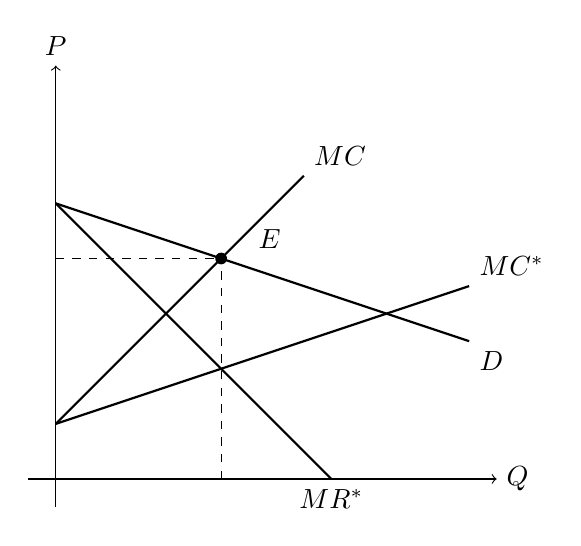
\begin{tikzpicture}[scale = 0.7]
                % Axes
                \draw[->] (-0.5,0) -- (8,0) node[right] {$Q$}; % Horizontal axis
                \draw[->] (0,-0.5) -- (0,7.5) node[above] {$P$}; % Vertical axis

                % Demand Curve (D_1) - passes through (0,5), (3,4), and (7.5,2.5)
                \draw[thick] (0,5) -- (7.5,2.5) node[below right] {$D$};
                % Marginal Revenue (MR_1) - passes through (0,5), (3,2), and (5,0)
                \draw[thick] (0,5) -- (5,0) node[below] {$MR^{*}$};

                % Supply Curve under competition (S^c) - passes through (0,1), (3,4), and (4.5,5.5)
                \draw[thick] (0,1) -- (4.5,5.5) node[above right] {$MC$};

                % Supply Curve under monopoly (S^m) - passes through (0,1), (3,2), and (7.5,3.5)
                \draw[thick] (0,1) -- (7.5,3.5) node[above right] {$MC^{*}$};

                % Equilibrium point (E_1) - intersection of D_1 and S^c at (3,4)
                \node[circle, fill, inner sep=1.5pt] (E1) at (3,4) {};
                \node[above right] at (E1) {$\quad E$};
                \draw[dashed] (3,0) -- (3,4);
                \draw[dashed] (0,4) -- (3,4);
            \end{tikzpicture}
            \caption{Step 1: Observable equivalence holds.}
            \label{fig:identification_example_step_1}
        \end{subfigure}
        \hfill
        \begin{subfigure}[b]{0.45\textwidth}
            \centering
            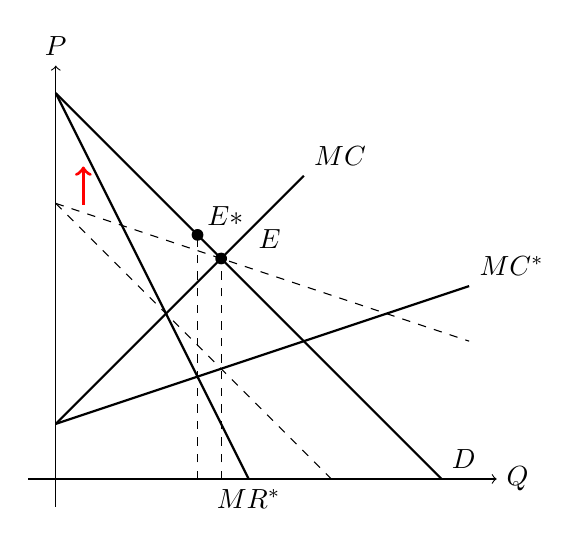
\begin{tikzpicture}[scale = 0.7]
                % Axes
                \draw[->] (-0.5,0) -- (8,0) node[right] {$Q$}; % Horizontal axis
                \draw[->] (0,-0.5) -- (0,7.5) node[above] {$P$}; % Vertical axis

                % Demand Curve (D_1) - passes through (0,5), (3,4), and (7.5,2.5)
                \draw[dashed] (0,5) -- (7.5,2.5) ;
                % Marginal Revenue (MR_1) - passes through (0,5), (3,2), and (5,0)
                \draw[dashed] (0,5) -- (5,0);


                % Shifted Demand Curve (D_1 shifted)
                \draw[thick] (0,7) -- (7,0) node[above right] {$D$};
                % Shifted MR (MR_1 shifted)
                \draw[thick] (0,7) -- (3.5,0) node[below] {$MR^{*}$};

                \draw[-<, very thick, red] (0.5,5) to[out=270,in=90] (0.5,5.5);


                % Supply Curve under competition (S^c) - passes through (0,1), (3,4), and (4.5,5.5)
                \draw[thick] (0,1) -- (4.5,5.5) node[above right] {$MC$};

                % Supply Curve under monopoly (S^m) - passes through (0,1), (3,2), and (7.5,3.5)
                \draw[thick] (0,1) -- (7.5,3.5) node[above right] {$MC^{*}$};

                % Equilibrium point (E_1) - intersection of D_1 and S^c at (3,4)
                \node[circle, fill, inner sep=1.5pt] (E1) at (3,4) {};
                \node[above right] at (E1) {$\quad E$};
                \draw[dashed] (3,0) -- (3,4);

                % Equilibrium point (E_2) - intersection of D_1 and S^c at (7/2,9/2)
                \node[circle, fill, inner sep=1.5pt] (E2) at (18/7,7 - 18/7) {};
                \node[above right] at (E2) {$E{*}$};
                \draw[dashed] (18/7,0) -- (18/7,7 - 18/7);
            \end{tikzpicture}
            \caption{Step 2: Demand rotation changes $D$ and $MR^{*}$}
            \label{fig:identification_example_step_2}
        \end{subfigure}
        \begin{subfigure}[b]{0.45\textwidth}
            \centering
            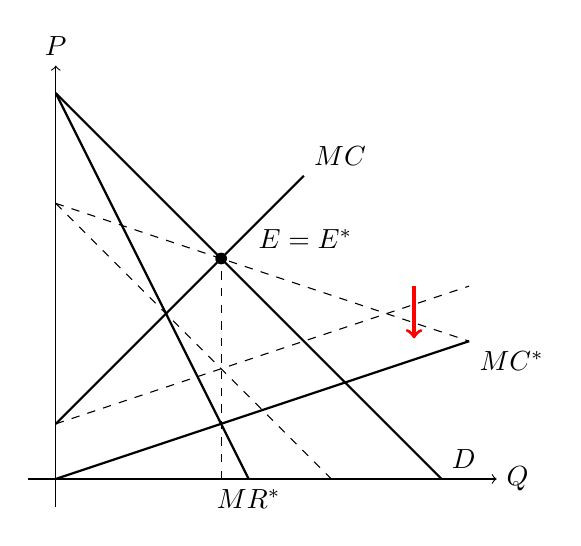
\begin{tikzpicture}[scale = 0.7]
                % Axes
                \draw[->] (-0.5,0) -- (8,0) node[right] {$Q$}; % Horizontal axis
                \draw[->] (0,-0.5) -- (0,7.5) node[above] {$P$}; % Vertical axis

                % Demand Curve (D_1) - passes through (0,5), (3,4), and (7.5,2.5)
                \draw[dashed] (0,5) -- (7.5,2.5) ;
                % Marginal Revenue (MR_1) - passes through (0,5), (3,2), and (5,0)
                \draw[dashed] (0,5) -- (5,0);

                % Shifted Demand Curve (D_1 shifted)
                \draw[thick] (0,7) -- (7,0) node[above right] {$D$};
                % Shifted MR (MR_1 shifted)
                \draw[thick] (0,7) -- (3.5,0) node[below] {$MR^{*}$};

                % Supply Curve under competition (S^c) - passes through (0,1), (3,4), and (4.5,5.5)
                \draw[thick] (0,1) -- (4.5,5.5) node[above right] {$MC$};

                % Supply Curve under monopoly (S^m) - passes through (0,1), (3,2), and (7.5,3.5)
                \draw[dashed] (0,1) -- (7.5,3.5);
                \draw[->, very thick, red] (6.5,3.5) -- (6.5,2.55);

                % Supply Curve under monopoly (S^m) - passes through (0,1), (3,2), and (7.5,3.5)
                \draw[thick] (0,0.0) -- (7.5,2.5) node[below right] {$MC^{*}$};

                % Equilibrium point (E_1) - intersection of D_1 and S^c at (3,4)
                \node[circle, fill, inner sep=1.5pt] (E1) at (3,4) {};
                \node[above right] at (E1) {$\quad E = E^{*}$};
                \draw[dashed] (3,0) -- (3,4);
            \end{tikzpicture}
            \caption{Step 3.1: The intercept of $MC^{*}$ changes along with the demand rotation to keep $E = E^{*}$.}
            \label{fig:identification_example_step_3_1}
        \end{subfigure}
        \hfill
        \begin{subfigure}[b]{0.45\textwidth}
            \centering
            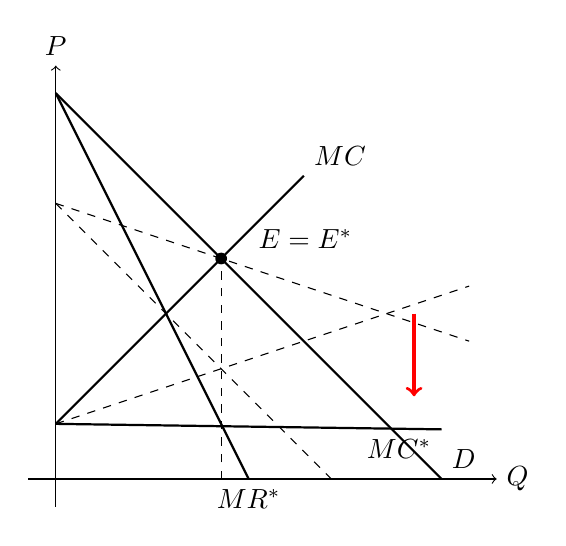
\begin{tikzpicture}[scale = 0.7]
                % Axes
                \draw[->] (-0.5,0) -- (8,0) node[right] {$Q$}; % Horizontal axis
                \draw[->] (0,-0.5) -- (0,7.5) node[above] {$P$}; % Vertical axis

                % Demand Curve (D_1) - passes through (0,5), (3,4), and (7.5,2.5)
                \draw[dashed] (0,5) -- (7.5,2.5) ;
                % Marginal Revenue (MR_1) - passes through (0,5), (3,2), and (5,0)
                \draw[dashed] (0,5) -- (5,0);

                % Shifted Demand Curve (D_1 shifted)
                \draw[thick] (0,7) -- (7,0) node[above right] {$D$};
                % Shifted MR (MR_1 shifted)
                \draw[thick] (0,7) -- (3.5,0) node[below] {$MR^{*}$};

                % Supply Curve under competition (S^c) - passes through (0,1), (3,4), and (4.5,5.5)
                \draw[thick] (0,1) -- (4.5,5.5) node[above right] {$MC$};

                % Supply Curve under monopoly (S^m) - passes through (0,1), (3,2), and (7.5,3.5)
                \draw[dashed] (0,1) -- (7.5,3.5);
                \draw[->, very thick, red] (6.5,3) -- (6.5,1.5);

                % Supply Curve under monopoly (S^m) - passes through (0,1), (3,2), and (7.5,3.5)
                \draw[thick] (0,1) -- (7,0.9) node[below left] {$MC^{*}$};

                % Equilibrium point (E_1) - intersection of D_1 and S^c at (3,4)
                \node[circle, fill, inner sep=1.5pt] (E1) at (3,4) {};
                \node[above right] at (E1) {$\quad E = E^{*}$};
                \draw[dashed] (3,0) -- (3,4);

            \end{tikzpicture}
            \caption{Step 3.2: The slope of $MC^{*}$ changes along with the demand rotation to keep $E = E^{*}$.}
            \label{fig:identification_example_step_3_2}
        \end{subfigure}
    \end{center}
    \caption{Intuition of the role of demand rotation instrument and identification}
    \label{fig:identification_example}
    \vspace{2mm}
    \footnotesize
    Note: The figures illustrate the intuition of how the demand rotation instrument works to identify the conduct parameter.
    $MC$ is the true marginal cost function, and $MC^{*}$ is the marginal cost function that rationalizes the monopoly conduct.
    Step 1 illustrates monopoly and perfect competition are observationally equivalent.
    In step 2, the demand rotation changes the intercept and slope of the demand function without changing the equilibrium point under perfect competition, but changes the equilibrium point under monopoly.
    Step 3 illustrates that to keep the equilibrium point under monopoly, $MC^{*}$ should change along with the demand rotation, which is impossible because the marginal cost function is independent of the demand shifter.
\end{figure}

In Figure \ref{fig:identification_example_step_1}, the perfect competition and the monopoly leads to the same equilibrium $E$.
Then, consider the change in the demand rotation instrument $X^{d}_1$.
In Figure \ref{fig:identification_example_step_2}, the demand rotation changes the intercept and slope of the demand function without changing the equilibrium point under the true model.
Under the monopoly, the new equilibrium point is $E^{*}$, which is different from $E$ and hence the observational equivalence is violated.
So as to lead to the same equilibrium after the change in the demand rotation ($E = E^{*})$, $MC^{*}$ should shift as in Figure \ref{fig:identification_example_step_3_1} and \ref{fig:identification_example_step_3_2}.
Note that we changed only the demand shifter, and hence the cost shifter $X^{s}$ is unchanged.
Thus, for observational equivalence to hold, the shift in $MC^{*}$ should be derived from the change in the demand rotation instrument, which implies that $MC^{*}$ is a function of the demand shifter.
However, this is impossible because it violates Assumption \ref{assumption:exclusive_shifters}, that is, the demand shifter should not affect the marginal cost function.

In Definition \ref{definition:non_identification}, non-identification requires to find two distinct pairs of a conduct parameter and a marginal cost function that lead to the same equilibrium quantity.
Here, we show only that the demand rotation breaks observational equivalence when the marginal cost is a linear function, and hence there is a possibility that observational equivalence can be achieved without depending on the demand shifter under non-linear marginal costs.
However, as we will see, when an inverse demand function includes demand shifter working as demand rotation instrument, for any marginal cost function, the marginal cost function under an alternative conduct parameter will be a function of the demand shifter, and hence the non-identification cannot hold.


\section{Characterization of Non-identification}\label{sec:nonidentification_characterization}

Hereafter, we provide an alternative result for the non-identification of the conduct parameter and the marginal cost function. 
First, we derive the necessary condition for non-identification based on Definition \ref{definition:non_identification}.
Then, we provide a transformation between marginal cost functions that leads to observational equivalence given an inverse demand function.
To make the transformation valid, we need to remove the effect of the demand shifter from the transformation, which put restrictions on the inverse demand function.
Then, we obtain the inverse demand function that is a necessary condition of the non-identification.
We then check that under the restricted inverse demand function, we can construct a transformation that leads to observational equivalence, which is the sufficient condition for non-identification.


\subsection{Necessary Condition for Non-identification}\label{subsec:necessary_condition_nonidentification}

First, we characterize the non-identification condition based on Definition \ref{definition:non_identification}.
The characterization is based on the fact that observational equivalence implies that the reduced form of the equilibrium quantity $h_q$ and $h_q^{*}$ are identical for any $X^{d}$ and $X^{s}$.
Therefore, its derivative with respect to the demand and cost shifters, $\nabla h_q$ and $\nabla h_q^{*}$, should be also identical.
Then, by applying the implicit function theorem to the equilibrium condition, we can compute $\nabla h_q$ and $\nabla h_q^{*}$.
The following lemma characterizes the non-identification condition:
\begin{lemma}\label{lemma:nonidentification_charaterization}
    Non-identification implies that for any $X^{d}$, $X^{s}$, and $Q^e$ under these exogenous variables, we have for $i = 1, \ldots, K_d$,
    \begin{align}
        &\frac{\partial P}{\partial X^{d}_{i}}(Q^e, X^{d}) + \theta^{*} Q^e \frac{\partial^2 P}{\partial X^{d}_{i}\partial Q}(Q^e, X^{d})\\  
        &= \lambda(Q^e, X^{d}, X^{s})\left[ \frac{\partial P}{\partial X^{d}_{i}}(Q^e, X^{d}) + \theta Q^e \frac{\partial^2 P}{\partial X^{d}_{i}\partial Q}(Q^e, X^{d}) \right], \label{eq:nonidentification_demand}
    \end{align}
    and for $j = 1,\ldots, K_s$,
    \begin{align}
        \frac{\partial MC^{*}}{\partial X^{s}_j}(Q^e, X^{s}) = \lambda(Q^e, X^{d}, X^{s}) \frac{\partial MC}{\partial X^{s}_j}(Q^e, X^{s}),\label{eq:nonidentification_marginal_cost}
    \end{align}
    where $\lambda(Q^e, X^{d}, X^{s})$ is defined as
    \begin{align}
        \lambda(Q^e, X^{d}, X^{s}) \equiv \frac{(1+\theta^{*})\frac{\partial P}{\partial Q}(Q^e, X^{d}) + \theta^{*} Q^e\frac{\partial^2 P}{\partial Q^2}(Q^e, X^{d}) - \frac{\partial MC^{*}}{\partial Q}(Q^e, X^{s})}{(1+\theta)\frac{\partial P}{\partial Q}(Q^e, X^{d}) + \theta Q^e\frac{\partial^2 P}{\partial Q^2}(Q^e, X^{d}) - \frac{\partial MC}{\partial Q}(Q^e, X^{s})}. \label{eq:lambda_foc}
    \end{align}
\end{lemma}
See Appendix \ref{appendix:proof} for the detailed proof.
Equation \eqref{eq:nonidentification_demand} and \eqref{eq:nonidentification_marginal_cost} imply that when non-identification holds, the derivative of the marginal revenue with $\theta$ can be transformed into the derivative of the marginal revenue with $\theta^{*}$, and the derivative of the marginal cost $MC$ with respect to $X^{s}$ can be transformed into the derivative of the marginal cost $MC^{*}$ with respect to $X^{s}$ by $\lambda(Q^e, X^{d}, X^{s})$.

These transformations cannot be always valid because the transformed marginal revenue is affected by cost shifter $X^{s}$, and the transformed marginal cost is affected by demand shifter $X^{d}$ through $\lambda(\cdot)$.
However, removing effect of $X^{s}$ from $\lambda(\cdot)$ is not appropriate because in this case, $\lambda(\cdot)$ depends only on $Q^e$ and $X^{d}$, and hence the transformation is not valid for the marginal cost.

To consider a valid transformation, we further rewrite \eqref{eq:nonidentification_demand} and \eqref{eq:nonidentification_marginal_cost}.
The next lemma provides a transformation of the derivative of $MC$ and $MC^{*}$ with respect to $Q$ and $X^{s}$ that leads to observational equivalence:
\begin{lemma}\label{lemma:mc_transformation}
    For any $Q^e$, $X^{d}$, and $X^{s}$, non-identification implies that the derivative of marginal cost $MC$ can be transformed into the derivative of marginal cost $MC^{*}$: for $i = 1, \ldots, K_d$, and $j = 1, \ldots, K_s$,
    \begin{align}
        \frac{\partial MC^{*}}{\partial Q}(Q^e, X^{s}) =D_i(Q^e, X^{d}) + C_i(Q^e, X^{d})\frac{\partial MC}{\partial Q}(Q^e, X^{s}),\label{eq:mc_transformation_quantity}
    \end{align}
    and
    \begin{align}
        \frac{\partial MC^{*}}{\partial X^{s}_j}(Q^e, X^{s}) = C_i(Q^e, X^{d})\frac{\partial MC}{\partial X^{s}_j}(Q^e, X^{s}).\label{eq:mc_transformation_cost_shifter},
    \end{align}
    where $C_i(Q, X^{d})$ and $D_i(Q, X^{d})$ are defined as
    \begin{align}
        C_i(Q, X^{d}) \equiv \frac{\frac{\partial P}{\partial X^{d}_i}(Q, X^{d}) + \theta^{*} Q\frac{\partial^2 P}{\partial X^{d}_{i}\partial Q}(Q, X^{d}) }{\frac{\partial P}{\partial X^{d}_i}(Q, X^{d}) + \theta Q\frac{\partial^2 P}{\partial X^{d}_{i}\partial Q}(Q, X^{d}) },\label{eq:ratio_marginal_revenue}
    \end{align}
    and
    \begin{align}
        D_i(Q, X^{d}) & \equiv\frac{\theta^{*} - \theta}{\frac{\partial P}{\partial X^{d}_i}(Q, X^{d}) + \theta Q\frac{\partial^2 P}{\partial X^{d}_{i}\partial Q}(Q, X^{d})}\Bigg[\frac{\partial P}{\partial Q}(Q, X^{d}) \frac{\partial P}{\partial X^{d}_i}(Q, X^{d})\\
        &\quad + Q\frac{\partial^2 P}{\partial Q^2}(Q, X^{d}) \frac{\partial P}{\partial X^{d}_i}(Q, X^{d}) - Q \frac{\partial P}{\partial Q}(Q, X^{d}) \frac{\partial^2 P}{\partial X^{d}_i\partial Q}(Q, X^{d}) \Bigg]\label{eq:intercation_derivative_demand}
    \end{align}
\end{lemma}
See Appendix \ref{appendix:proof} for the detailed proof.
The subscript $i$ in $C_i$ and $D_i$ indicates that $C_i$ and $D_i$ consist of the derivative of the inverse demand function with respect to $X^{d}_i$.
Unlike Lemma \ref{lemma:nonidentification_charaterization}, we have only the transformation relating to marginal cost, and hence we can see the problem in this transformation clearly. 
As we saw in Section \ref{sec:lau_result}, for the transformations to hold universally for any $Q^e$ and $X^{s}$, they must be independent of $X^{d}$.
If the dependence holds, while demand rotation does not change the equilibrium quantity $Q^e$, it changes $MC^{*}$ via $C_i$ and $D_i$, which violates Assumption \ref{assumption:exclusive_shifters}. 
Therefore, in order for the transformations to be valid, both $C_i$ and $D_i$ must be independent of $X^{d}$.

The terms $C_i$ and $D_i$ are independent of $X^{d}$ when the derivative of the inverse demand function with respect to $X^{d}_i$ is zero.
A concern is that as $C_i$ and $D_i$ already consist of the second-order derivative of inverse demand function, to take the derivative of $C_i$ and $D_i$, we need a strong restriction on the inverse demand function.
The following assumption is necessary for this purpose:
\begin{assumption}\label{assumption:three_times_differentiable}
    The inverse demand function is three times continuously differentiable.
    The marginal cost function is twice continuously differentiable.
\end{assumption}
This assumption puts a stronger restriction on the inverse demand function than Assumption \ref{assumption:twice_differentiable}.
Actually, while Lau impose only the twice-continuous differentiability, we will discuss that his proof potentially requires three-times differentiability on the inverse demand function.
Therefore, to characterize the non-identification condition, Assumption \ref{assumption:three_times_differentiable} is inevitable.


Before we characterize the inverse demand function that makes $C_i$ and $D_i$ independent of $X^{d}$, we first check when $C_i$ and $D_i$ are not well-defined.
This implies that \eqref{eq:ratio_marginal_revenue} and \eqref{eq:intercation_derivative_demand} are violated, and hence the identification holds by Definition \ref{definition:identification}.
All derivatives in $C_i$ and $D_i$ are finite by Assumption \ref{assumption:three_times_differentiable}, and hence the numerator and the denominator of $C_i$ and $D_i$ cannot take infinite values.
In this case, no matter what value of the numerator of $C_i$ and $D_i$ is, \eqref{eq:ratio_marginal_revenue} and \eqref{eq:intercation_derivative_demand} are violated when at least one of the denominator of $C_i$ and $D_i$ for $i= 1, \ldots, K_d$ is zero, under which $C_i$ and $D_i$ will be infinite or indeterminate.



This implies that for any $Q$ and $X^{d}$, and for some $i$, 
\begin{align}
    \frac{\partial P}{\partial X^{d}_i}(Q, X^{d}) + \theta Q\frac{\partial^2 P}{\partial X^{d}_{i}\partial Q}(Q, X^{d}) = 0. \label{eq:identification_condition_separable}
\end{align}
Let $\mathcal{I}$ be the set of indices of the demand shifters where \eqref{eq:identification_condition_separable} holds.
Then, by \eqref{eq:identification_condition_separable}, we can characterize the inverse demand function that always leads to identification:
\begin{lemma}\label{lemma:identification_condition_separable}
    Suppose that $\theta \ne 0$.
    Then, the conduct parameter and the marginal cost function are identified when the inverse demand function is such that
    \begin{align}
        P(Q, X^{d}) = Q^{-\frac{1}{\theta}}r(X^{d}) + s(Q, X^{d}_{-\mathcal{I}}), \label{eq:identification_separable_demand}
    \end{align}
    where $X^{d}_{-\mathcal{I}}$ is the vector of demand shifters whose index is not in $\mathcal{I}$, and $r(\cdot)$ and $s(\cdot)$ are twice continuously differentiable functions.
\end{lemma}
See Appendix \ref{appendix:proof} for the proof.
To get the intuition why \eqref{eq:identification_condition_separable} leads to the identification, note that \eqref{eq:identification_condition_separable} can be rewritten as
\begin{align}
    \frac{\partial }{\partial X^{d}_i}\left( P(Q, X^{d}) + \theta Q \frac{\partial P}{\partial Q}(Q, X^{d})\right) = 0,
\end{align}
which is the derivative of the marginal revenue under $\theta$ with respect to $X^{d}_i$.
Additionally, under \eqref{eq:identification_separable_demand}, the equilibrium condition \eqref{eq:foc_theta} is given as
\begin{align}
    s(Q, X^{d}_{-\mathcal{I}}) + \theta Qs'(Q, X^{d}_{-\mathcal{I}}) = MC(Q, X^{s}),
\end{align}
Therefore, both imply that when \eqref{eq:identification_condition_separable} holds, the equilibrium quantity is not affected by the change in $X^{d}_i$, and hence $X^{d}_i$ always work as a demand rotation instrument under $\theta$.
On the other hand, for any other $\theta^{*} \ne \theta$, the equilibrium condition becomes
\begin{align}
    Q^{-\frac{1}{\theta}}r(X^{d})\left(1 - \frac{\theta}{\theta^{*}}\right) + s(Q, X^{d}_{-\mathcal{I}}) +  Qs'(Q, X^{d}_{-\mathcal{I}}) = MC(Q, X^{s}).
\end{align}
As $r(X^{d})$ is a function of $X^{d}_i$ and  $r(X^{d})$ is not a constant by Assumption \ref{assumption:exclusive_shifters}, the equilibrium condition implies that the equilibrium quantity should depend on $X^{d}_i$ under $\theta^{*}$.
Therefore, while the change in $X^{d}_i$ does not change the equilibrium quantity under $\theta$, it changes under $\theta^{*}$, which violates observationally equivalence.
Therefore, the conduct parameter and the marginal cost function are identified.


Now, suppose that \eqref{eq:identification_condition_separable} does not hold for all demand shifters.
Then, we can characterize the inverse demand functions where $C_i$ and $D_i$ are independent of $X^{d}$.
The following proposition shows that there is an inverse demand function that satisfies this condition:
\begin{proposition}\label{proposition:nonidentification_inverse_demand}
    Suppose that \eqref{eq:identification_condition_separable} does not hold for any $i = 1, \ldots, K_d$.
    Then, $C_i(Q, X^{d})$ and $D_i(Q, X^{d})$ are independent of $X^{d}$ if and only if the inverse demand function is given as \begin{align}
        P(Q, X^{d}) = Q^{\alpha_1}r(X^{d}) + s(Q), \label{eq:nonidentification_inverse_demand}
    \end{align}
    where $\alpha_1 \ne -\frac{1}{\theta}$ is a constant, and $r(\cdot)$ and $s(\cdot)$ are twice continuously differentiable functions.
\end{proposition}
See Appendix \ref{appendix:proof} for the proof.
As in Theorem \ref{theorem_lau}, non-identification implies separable inverse demand functions.
However, our result tells more about under what type of separable function the non-identification holds.
Observe that when $\alpha_1 \ne 0$, the demand shifter changes only the slope of the inverse demand function, and when $\alpha_1 = 0$, the demand shifter changes only the intercept of the inverse demand function.
Therefore, we cannot have any demand rotation instrument under \eqref{eq:nonidentification_inverse_demand}.
The contrapositive of Proposition \ref{proposition:nonidentification_inverse_demand} implies that whenever we have a set of demand shifters that can work as demand rotation instrument, the conduct parameter and the marginal cost function are identified.
This emphasizes the idea of \citet{bresnahanOligopoly1982} in more general setting.

Additionally, unlike in Theorem \ref{theorem_lau}, our result implies that the dimension of the demand shifter does not matter for the identification because our result holds for any dimension of the demand shifter.
Recall that the inverse demand function \eqref{eq:demand_counterexample} is separable, but $X^{d}$ can work as a demand rotation instrument.
In this case, $C_i$ and $D_i$ are given as
\begin{align}
    C_i(Q, X^{d}) = \frac{\alpha_2 + \theta\alpha_3Q}{\alpha_2 + \theta^{*}\alpha_3Q}\quad \text{ and }\quad  D_i(Q, X^{d}) =  (\theta^{*} - \theta)(-\alpha_1 + \alpha_3X^{d}).
\end{align}
This implies that the transformation \eqref{eq:mc_transformation_quantity} is not valid for any marginal cost function because $D_i(Q, X^{d})$ depends on $X^{d}$.
Therefore, any $MC^{*}$ that leads to observational equivalence with $MC$ should depend on the demand shifter, under which non-identification is impossible.
While Figure \ref{fig:identification_example} considers the case where the marginal cost function is linear, Proposition \ref{proposition:nonidentification_inverse_demand} implies that \eqref{eq:demand_counterexample} can identify the conduct parameter and the marginal cost in more general setting.
Hence, whether the inverse demand function is separable or not is not enough for the identification, and the demand rotation instrument is the key for the identification.




\subsubsection{Discussions}\label{subsubsec:necessary_condition_discussion}

Before moving to the sufficient condition for non-identification, we discuss the problem in Lau's proof.
To show Theorem \ref{theorem_lau}, Lau follows the same logic as in Lemma \ref{lemma:nonidentification_charaterization}, but he obtains a slightly different equation from \eqref{eq:nonidentification_marginal_cost}:
\begin{align}
    \frac{\partial MC^{*}}{\partial X^{s}_j}(Q, X^{s}) = \lambda'(Q, X^{s}) \frac{\partial MC}{\partial X^{s}_j}(Q, X^{s}),\quad \forall Q, X^{s}, \label{eq:nonidentification_marginal_cost_lau}
\end{align}
where $\lambda'(Q, X^{s})$ depends only on $Q$ and $X^{s}$.
This corresponds to Equation (15) in \citet{lauIdentifying1982}.
Then he concludes that there is a transformation $T$ such that 
\begin{align}
    MC^{*}(Q^e, X^{s}) = T(MC(Q^e, X^{s}), Q^e). \label{eq:mc_transformation_lau}
\end{align}
The existence of the transformation $T$ is shown by integrating \eqref{eq:nonidentification_marginal_cost_lau} with respect to $X^{s}$ when $X^{s}$ is a scalar, and by applying Lemma \ref{lemma_1_GU} from \citet{goldmanNote1964} when $X^{s}$ is a vector.

Lau's argument has several problems.
In our approach, both \eqref{eq:nonidentification_demand} and \eqref{eq:nonidentification_marginal_cost} are necessary to derive the transformation between marginal cost functions. 
It can be verified that Lau derives both equations \eqref{eq:nonidentification_demand} and \eqref{eq:nonidentification_marginal_cost} in his proof.
However, Lau relies solely on \eqref{eq:nonidentification_marginal_cost}, which limits the scope of his derivation.

Next, Lau does not explicitly define $\lambda'(\cdot)$ in his formulation, but it can be inferred that his $\lambda'(\cdot)$ corresponds to $\lambda(\cdot)$.
However, he neglects a point that the function $\lambda'(\cdot)$ implicitly depends on the demand shifter $X^{d}$, and this dependence is not addressed in his analysis.
As long as the variable $X^d$ cannot be eliminated from $\lambda'(\cdot)$, the transformation $T$ between $MC$ and $MC^*$ will necessarily depend on $X^d$, contradicting Assumption \ref{assumption:exclusive_shifters}.
Lau does not provide a justification for why $X^d$ can be removed from this expression, and hence it leaves a critical gap in the argument.

Furthermore, Lau assumes that the functions are twice continuously differentiable, which allows him to apply Lemma \ref{lemma_1_GU} to justify the existence of the transformation $T$. 
However, this reasoning is flawed because equation \eqref{eq:nonidentification_marginal_cost_lau} potentially retains dependence on $X^d$. 
To validly eliminate $X^d$, it is necessary to differentiate $\lambda(\cdot)$ with respect to $X^d$ and require that the derivative vanishes. 
This step, in turn, demands that the inverse demand function be at least three-times continuously differentiable as in our proof.




\subsection{Sufficient Condition for Non-identification}\label{subsec:sufficient_condition_nonidentification}
Because we characterize the inverse demand function implied by non-identification, we are interested in whether the inverse demand function can lead to the non-identification.
To see whether the inverse demand function \eqref{eq:nonidentification_inverse_demand} can lead to non-identification, we need to check whether there exists a transformation between the equilibrium conditions under $(\theta, MC)$ and $(\theta^{*}, MC^{*})$.
Then, when an equilibrium quantity $Q^e$ satisfies the equilibrium condition under $(\theta, MC)$, by applying the transformation to the equilibrium condition under $(\theta, MC)$, we have that
\begin{align}
    T\left(P(Q^e, X^{d}) + \theta Q^e \frac{\partial P}{\partial Q}(Q^e, X^{d}), Q^e\right)&= T\left(MC(Q^e, X^{s}), Q^e\right)\\
    P(Q^e, X^{d}) + \theta^{*} Q^e \frac{\partial P}{\partial Q}(Q^e, X^{d})&= MC^{*}(Q^e, X^{s}).
\end{align}
Thus, $Q^e$ also satisfies the equilibrium condition under $(\theta^{*}, MC^{*})$.

In fact, \eqref{eq:mc_transformation_quantity} can give us a sufficient condition for non-identification, that is, by using the inverse demand function \eqref{eq:nonidentification_inverse_demand}, we can construct the transformation for the equilibrium conditions.
\begin{proposition}\label{proposition:sufficient_nonidentification}
    Given the inverse demand function \eqref{eq:nonidentification_inverse_demand} where $\alpha_1 \ne -\frac{1}{\theta}$, there exists a transformation $T$ between the equilibrium conditions under $(\theta, MC)$ and $(\theta^{*}, MC^{*})$.
    Therefore, non-identification of the conduct parameter and the marginal cost function holds under \eqref{eq:nonidentification_inverse_demand}.
\end{proposition}
The proof is given in Appendix \ref{appendix:proof}.
Proposition \ref{proposition:sufficient_nonidentification} shows that more specific separable inverse demand function can lead to a transformation that leads to non-identification.
While Proposition \ref{proposition:sufficient_nonidentification} explicitly constructs the transformation that leads to observable equivalence,  Lau's sufficiency proof is incomplete because it implicitly assumes that there exists a transformation $T$ under a separable inverse demand function \eqref{eq:separable_demand}.
However, separability itself does not guarantee the existence of the transformation.







\subsection{Identification of the Inverse Demand Function}\label{sec:identification_inverse_demand}
So far, as in \citet{lauIdentifying1982}, we have characterized the non-identification problem given an inverse demand function, and hence we have not discussed the identification of the inverse demand function.
While Lau does not discuss the identification of the inverse demand function, he assumes that the reduced-form of the equilibrium quantity and the equilibrium price are identified:
\begin{assumption}\label{assumption:reduced_form}
    The reduced-form of the equilibrium quantity and the equilibrium price are identified:
    \begin{align}
        Q^e = h_q(X^{d}, X^{s}), \quad P^e = h_p(X^{d}, X^{s}).
    \end{align}
\end{assumption}
This is due to the variation in the demand and cost shifters.
However, this does not imply that the inverse demand function is identified.
Therefore, we need to consider whether the inverse demand function where the conduct parameter and the marginal cost function are not identified, can be identified.
When the inverse demand function is not identified, all components in the conduct parameter model cannot be identified.
Unfortunately, we have the following result:
\begin{proposition}\label{proposition:nonidentification_inverse_demand_with_nonidentifed_conduct_parameter}
    An inverse demand function cannot be identified when it has the following form:
    \begin{align}
        P(Q, X^{d}) = Q^{\alpha_1}r(X^{d}) + s(Q),
    \end{align}
    where $\alpha_1$ is a constant, and $r(\cdot)$ and $s(\cdot)$ are twice continuously differentiable functions.
\end{proposition}
See Appendix \ref{appendix:proof} for the proof.
It shows that for any $s(Q)$, another function $\tilde{s}(Q) = s(Q) + C Q^{-\frac{1}{\theta}}$ lead to the same equilibrium quantity for any $X^{d}$ and $X^{s}$, which implies that the inverse demand function itself is not identified.
Note that here $\alpha_1$ also include the case where $\alpha_1 = -\frac{1}{\theta}$.
Therefore, while Theorem \ref{theorem_lau} shows that the conduct parameter and the marginal cost function are identified as all demand shifters work as demand rotation instrument, the inverse demand function \eqref{eq:identification_separable_demand_lau} cannot be identified.

Another unfortunate news is that demand rotation instruments do not help to identify an inverse demand function with demand rotation instruments.
The following example demonstrate this point, and hence demand rotation instrument is not a necessary condition for the identification of the inverse demand function:
\begin{example}\label{example:demand_rotation_instrument_does_not_help_identification}
    Suppose the inverse demand function is given as
    \begin{align}
        P(Q, X^{d}) = Q^{\alpha_1}r(X^{d}) + s(Q) + t(X^{d}).
    \end{align}
    Here, $X^{d}$ works as demand rotation instrument through $r(\cdot)$ and $t(\cdot)$.
    However, in the same ways as in Proposition \ref{proposition:nonidentification_inverse_demand_with_nonidentifed_conduct_parameter}, it is easy to see that inverse demand functions with $s(Q)$ and $\tilde{s}(Q) = s(Q) + C Q^{-\frac{1}{\theta}}$ lead to the same equilibrium quantity, which implies that the inverse demand function is not identified.
\end{example}





\section{Main Result and Discussion}\label{sec:main_result_and_discussion}
Based on the results so far, we can summarize the main result.
First, Proposition \ref{proposition:nonidentification_inverse_demand} and Proposition \ref{proposition:sufficient_nonidentification} characterize the inverse demand function that leads to non-identification:
\begin{theorem}\label{theorem:identification_characterization}
    Given Assumption \ref{assumption:exclusive_shifters}, \ref{assumption:unique_equilibrium}, and \ref{assumption:three_times_differentiable}, the conduct parameter $\theta$ cannot be identified from data on price, quantity, and other exogenous variables alone if and only if the industry inverse demand function is given as
    \begin{align}
        P(Q, X^{d}) = Q^{\alpha_1}r(X^{d}) + s(Q)
    \end{align}
    where $\alpha_1 \ne -\frac{1}{\theta}$ is a constant, and $r(\cdot)$ and $s(\cdot)$ are twice continuously differentiable functions.
\end{theorem}

Second, while Lau assumes that the identification of the inverse demand function, Proposition \ref{proposition:nonidentification_inverse_demand_with_nonidentifed_conduct_parameter} shows that the inverse demand function that leads to non-identification cannot be identified.
Therefore, the all components in the conduct parameter model cannot be identified.
Additionally, Example \ref{example:demand_rotation_instrument_does_not_help_identification} shows that demand rotation instrument does not guarantee the identification of an inverse demand function.
Therefore, at least Theorem \ref{theorem:identification_characterization} implies that given an identified inverse demand function with demand rotation instrument, the conduct parameter and the marginal cost function can be nonparametrically identified.
This gives us the following corollary for the identification of the conduct parameter model:
\begin{corollary}\label{corollary:identification_conduct_parameter_model}
    When the inverse demand function with demand rotation instrument is identified, the conduct parameter and the marginal cost function are identified.
\end{corollary}




\subsection{Discussion}\label{subsec:main_result_discussion}
The results so far are true whenever we admit the conduct parameter approach.
In contrast, the conduct parameter approach has been criticized by several papers.
In this section, We discuss the micro-foundations of the conduct parameter approach and the accuracy of the conduct parameter approach.

\paragraph{Micro-foundations of Conduct Parameter Approach}
The conduct parameter approach is based on the conjectural variation model.
In the conjectural variation model, each firm has a conjecture about how the competitors will react to the firm's action.
A major problem of the conjectural variation model is that the conjecture and the reaction function does not coincide at the equilibrium.
\citet{bresnahanDuopoly1981,bresnahanExistence1983}  propose a Consistent Conjecture Equilibrium (CCE) which requires that the consistency between the conjecture and the reaction function is satisfied at the equilibrium.
However, the existence and uniqueness of the CCE is not guaranteed in general \citep{klempererConsistent1988,robsonExistence1983}.

However, several alternative micro-foundations have been proposed.
For example, \citet{escrihuela-villarNote2015} shows that corporation coefficient approach is equivalent to the conjectural variation model in some specific setting.
In this model, each firm maximizes its profit plus the weighted sum of its competitors profit, where the weight is called the corporation coefficient.
\citet{menezesStrategic2020} investigates the supply function approach where firms choose not quantity but supply schedule based on price.
\citet{menezesCompetition2023} show the relationship between the conduct parameter approach and the supply function approach in linear demand and linear marginal cost model case, and \citet{menezesStrategic2020} briefly discuss how to estimate the competitiveness given the information of marginal cost.

%\citet{adachiMicrofoundation2023} considers a micro-foundation where the representative firm chooses a quantity that equate a discounted marginal gain by $\theta$ and marginal loss.
%This condition is equivalent to the equilibrium condition in our model.
%However, his equilibrium condition is not derived as the first-order condition of the representative firm's profit maximization problem.


\paragraph{Accuracy of the Conduct Parameter Approach}
While this paper only focus on the identification problem, \citet{cortsConduct1999} criticize that the conduct parameter approach can be inaccurate when the data generation process is out of the conduct parameter model.
For example, a repeated game model can sustain the equilibrium quantity under the joint-profit maximization , the conduct parameter estimate will be biased from $\theta = 1$.
At least, as \citet{cortsConduct1999} and \citet{magnolfiComparison2022} mention, the critics can be avoided by assuming the data generation process is a static competition and derived from the equilibrium condition in \eqref{eq:foc}.


\section{Conclusion}\label{sec:conclusion}

This paper revisited the identification of the conduct parameter in homogeneous product market.
In the literature, Lau considers the identification problem in a fairly generalized setting.
While \citet{lauIdentifying1982} characterizes the non-identification condition, we point out some problems in Lau's paper and provide a novel characterization of the non-identification condition.
Based on the new characterization, we find that the non-identification is equivalent to the absence of demand shifters that works as demand rotation instrument proposed in \citet{bresnahanOligopoly1982}.
We then consider the identification of the all primitives in the model and show that when some demand shifters always work as demand rotation instruments, the inverse demand function cannot be identified, which immediately implies that the conduct parameter and the marginal cost function are also not identified.
Therefore, while demand rotation instrument is a key for the identification of the conduct parameter, it could be prevent us from the identification.



\paragraph{Acknowledgments}
This paper is based on Chapter 3 of the first author's dissertation submitted to Rice University.
We thank Jeremy Fox for his valuable advice.
We also thank to the participants of Professor Fox's group meeting for their helpful comments.



\bibliographystyle{aer}
\bibliography{conduct_parameter_counter_example}


\newpage
\appendix
\appendixsection
\numberwithin{theorem}{section}
\numberwithin{lemma}{section}
\numberwithin{proposition}{section}
\numberwithin{corollary}{section}
\numberwithin{definition}{section}
\numberwithin{example}{section}
\numberwithin{assumption}{section}
\numberwithin{claim}{section}

\begin{center}
\huge\textbf{Appendix}
\end{center}
\vspace{1mm}

\section{Omitted Proofs}\label{appendix:proof}
In this section, we provide the proofs of the lemmas and theorems in the main text.
In what follows, we suppress the arguments of functions when no confusion arises.


\subsection{Proof of Lemma \ref{lemma:nonidentification_charaterization}}
Assume that given $X^{d}$ and $X^{s}$, we can solve the equilibrium condition for the equilibrium quantity $Q^e$.
For notational simplicity, we define
\begin{align}
    F(Q^e, X^{d}, X^{s}; \theta, MC) \equiv P(Q^e, X^{d}) + \theta Q^e\frac{\partial P}{\partial Q}(Q^e, X^{d}) - MC(Q^e, X^{s}).
\end{align}
Then, by Assumption \ref{assumption:unique_equilibrium}, we can apply the implicit function theorem, and for the reduced-form equation $Q^e = h_q(X^{d}, X^{s})$, the gradient of the reduced-form function $h_q$ with respect to $X^{d}$ and $X^{s}$ is given by
\begin{align}
    \nabla h_q(X^{d}, X^{s}) =  \left( -\dfrac{\frac{\partial F}{\partial X^{m}_{i}}(h_q(X^{d}, X^{s}), X^{d}, X^{s})}{\frac{\partial F}{\partial Q}(h_q(X^{d}, X^{s}), X^{d}, X^{s})} \right)_{\substack{m = d, s\\ i = 1, \ldots, K_m}}. \label{eq:foc_derivative_demand_supply}
\end{align}
The derivatives of $F$ for each variable are for $i = 1, \ldots, K_d$ and $i = 1, \ldots, K_s$,
\begin{align}
    \frac{\partial F}{\partial X^{d}_i}(Q^e, X^{d}, X^{s}; \theta, MC) & =  \frac{\partial P}{\partial X^{d}_{i}}(Q^e, X^{d}) + \theta\frac{\partial^2 P}{\partial X^{d}_{i}\partial Q}(Q^e, X^{d})Q^e,\\
    \frac{\partial F}{\partial X^{s}_i}(Q^e, X^{d}, X^{s}; \theta, MC) & =  -\frac{\partial MC}{\partial X^{s}_{i}}(Q^e, X^{s}), \\
    \frac{\partial F}{\partial Q}(Q^e, X^{d}, X^{s}; \theta, MC) & = (1+\theta)\frac{\partial P}{\partial Q}(Q^e, X^{d}) + \theta Q^e\frac{\partial^2 P}{\partial Q^2}(Q^e, X^{d}) - \frac{\partial MC}{\partial Q}(Q^e, X^{s}).
\end{align}
Thus, the derivative of $h$ with respect to $X^{d}_i$ and $X^{s}_i$ are given as for $i = 1, \ldots, K_d$ and $i = 1, \ldots, K_s$,
\begin{align}
    \frac{\partial h_q}{\partial X^{d}_{i}}(X^{d}, X^{s}) = -\frac{\frac{\partial P}{\partial X^{d}_{i}}(Q^e, X^{d}) + \theta Q^e \frac{\partial^2 P}{\partial X^{d}_{i}\partial Q}(Q^e, X^{d}) }{(1+\theta)\frac{\partial P}{\partial Q}(Q^e, X^{d}) + \theta  Q^e\frac{\partial^2 P}{\partial Q^2}(Q^e, X^{d}) - \frac{\partial MC}{\partial Q}(Q^e, X^{s})}, \label{eq:foc_derivative_demand}
\end{align}
and
\begin{align}
    \frac{\partial h_q}{\partial X^{s}_{i}}(X^{d}, X^{s}) & = \frac{\frac{\partial MC}{\partial X^{s}_{i}}(Q^e, X^{s})}{(1+\theta)\frac{\partial P}{\partial Q}(Q^e, X^{d}) + \theta  Q^e\frac{\partial^2 P}{\partial Q^2}(Q^e, X^{d}) - \frac{\partial MC}{\partial Q}(Q^e, X^{s})}. \label{eq:foc_derivative_supply}
\end{align}

% Use the definition of non-identification
Note that the same argument can be applied to the equilibrium condition \eqref{eq:foc_theta_star} of the alternative model.
Recall that the non-identification implies that $Q^e = h_q(X^{d}, X^{s}) = h_q^{*}(X^{d}, X^{s})$ for all $X^{d}$ and $X^{s}$, and hence we must have
\begin{align}
    \nabla h_q^{*}(X^{d}, X^{s}) = \nabla h_q(X^{d}, X^{s}) \quad \forall X^{d}, X^{s}. \label{eq:observale_equivalence_derivative}
\end{align}
From \eqref{eq:foc_derivative_demand_supply}, this implies that for all $Q^e$, $X^{d}$, and $X^{s}$,
\begin{align}
    \begin{pmatrix}
        \frac{\partial F}{\partial X^{d}_{1}}(Q^e, X^{d}, X^{s}; \theta^{*}, MC^{*})\\
        \vdots \\
        \frac{\partial F}{\partial X^{d}_{K_d}}(Q^e, X^{d}, X^{s}; \theta^{*}, MC^{*})\\
        \frac{\partial F}{\partial X^{s}_{1}}(Q^e, X^{d}, X^{s}; \theta^{*}, MC^{*})\\
        \vdots \\
        \frac{\partial F}{\partial X^{s}_{K_s}}(Q^e, X^{d}, X^{s}; \theta^{*}, MC^{*})
    \end{pmatrix}
    = \lambda(Q^e, X^{d}, X^{s})
    \begin{pmatrix}
        \frac{\partial F}{\partial X^{d}_{1}}(Q^e, X^{d}, X^{s}; \theta, MC)\\
        \vdots \\
        \frac{\partial F}{\partial X^{d}_{K_d}}(Q^e, X^{d}, X^{s}; \theta, MC)\\
        \frac{\partial F}{\partial X^{s}_{1}}(Q^e, X^{d}, X^{s}; \theta, MC)\\
        \vdots \\
        \frac{\partial F}{\partial X^{s}_{K_s}}(Q^e, X^{d}, X^{s}; \theta, MC)
    \end{pmatrix},\label{eq:foc_derivative_demand_supply_lambda}
\end{align}
where $\lambda(Q^e, X^{d}, X^{s})$ is defined as
\begin{align}
    \lambda(Q^e, X^{d}, X^{s}) \equiv \frac{(1+\theta^{*})\frac{\partial P}{\partial Q}(Q^e, X^{d}) + \theta^{*} Q^e\frac{\partial^2 P}{\partial Q^2}(Q^e, X^{d}) - \frac{\partial MC^{*}}{\partial Q}(Q^e, X^{s})}{(1+\theta)\frac{\partial P}{\partial Q}(Q^e, X^{d}) + \theta Q^e\frac{\partial^2 P}{\partial Q^2}(Q^e, X^{d}) - \frac{\partial MC}{\partial Q}(Q^e, X^{s})}.
\end{align}
Assumption \ref{assumption:unique_equilibrium} guarantees that $\lambda(Q^e, X^{d}, X^{s})$ is nonzero and finite.
From the first $K_d$ rows in \eqref{eq:foc_derivative_demand_supply_lambda}, \eqref{eq:nonidentification_demand} and for the later $K_s$ rows, \eqref{eq:nonidentification_marginal_cost} hold.


\subsection{Proof of Lemma \ref{lemma:mc_transformation}}

From \eqref{eq:nonidentification_demand}, we have (we suppress the arguments of the functions for brevity)
\begin{align}
    &\left[\frac{\partial P}{\partial X^{d}_i} + \theta^{*} Q^e\frac{\partial^2 P}{\partial X^{d}_{i}\partial Q}\right]\left[(1+\theta)\frac{\partial P}{\partial Q} + \theta Q^e\frac{\partial^2 P}{\partial Q^2} - \frac{\partial MC}{\partial Q}\right] \\
    & \hspace{4cm}= \left[\frac{\partial P}{\partial X^{d}_i} + \theta Q^e\frac{\partial^2 P}{\partial X^{d}_{i}\partial Q}\right]\left[(1+\theta^{*})\frac{\partial P}{\partial Q} + \theta^{*} Q^e\frac{\partial^2 P}{\partial Q^2} - \frac{\partial MC^{*}}{\partial Q}
    \right]\\
    & \frac{\frac{\partial P}{\partial X^{d}_i} + \theta^{*} Q\frac{\partial^2 P}{\partial X^{d}_{i}\partial Q} }{\frac{\partial P}{\partial X^{d}_i} + \theta Q\frac{\partial^2 P}{\partial X^{d}_{i}\partial Q} }\left[(1+\theta)\frac{\partial P}{\partial Q} + \theta Q^e\frac{\partial^2 P}{\partial Q^2} - \frac{\partial MC}{\partial Q}\right]\\
    &\hspace{4cm} =\left[(1+\theta^{*})\frac{\partial P}{\partial Q} + \theta^{*} Q^e\frac{\partial^2 P}{\partial Q^2} - \frac{\partial MC^{*}}{\partial Q}
    \right]\\
    & \frac{\partial MC^{*}}{\partial Q} = \underbrace{(1+\theta^{*})\frac{\partial P}{\partial Q} + \theta^{*} Q^e\frac{\partial^2 P}{\partial Q^2} - C_i(Q, X^{d}) \left[(1+\theta)\frac{\partial P}{\partial Q} + \theta Q^e\frac{\partial^2 P}{\partial Q^2} \right]}_{(\ast)} + C_i(Q, X^{d})\frac{\partial MC}{\partial Q}.
\end{align}
The terms in $(\ast)$ can be more simplified as 
\begin{align}
    &(1+ \theta^{*})\frac{\partial P}{\partial Q} + \theta^{*} Q\frac{\partial^2 P}{\partial Q^2} - \frac{\frac{\partial P}{\partial X^{d}_i} + \theta^{*} Q\frac{\partial^2 P}{\partial X^{d}_{i}\partial Q} }{\frac{\partial P}{\partial X^{d}_i} + \theta Q\frac{\partial^2 P}{\partial X^{d}_{i}\partial Q} }\left[(1+ \theta) \frac{\partial P}{\partial Q} + \theta Q\frac{\partial^2 P}{\partial Q^2}\right]\\
    &= \frac{1}{\frac{\partial P}{\partial X^{d}_i} + \theta\frac{\partial^2 P}{\partial X^{d}_{i}\partial Q}Q}\Bigg[\left((1 + \theta^{*}) \frac{\partial P}{\partial Q} + \theta^{*} Q\frac{\partial^2 P}{\partial  Q^2}\right)\left(\frac{\partial P}{\partial X^{d}_i} + \theta Q\frac{\partial^2 P}{\partial X^{d}_{i}\partial Q}\right)\\
    &\hspace{4cm} - \left( (1 + \theta) \frac{\partial P}{\partial Q} + \theta Q\frac{\partial^2 P}{\partial Q^2}\right)\left(\frac{\partial P}{\partial X^{d}_i} + \theta^{*} Q\frac{\partial^2 P}{\partial X^{d}_{i}\partial Q}\right)\Bigg]\\
    & =  \frac{\theta^{*} - \theta}{\frac{\partial P}{\partial X^{d}_i} + \theta\frac{\partial^2 P}{\partial X^{d}_{i}\partial Q}Q}\left[ \frac{\partial P}{\partial Q} \frac{\partial P}{\partial X^{d}_i} + Q\frac{\partial P}{\partial X^{d}_i}\frac{\partial^2 P}{\partial^2 Q} - Q\frac{\partial P}{\partial Q}\frac{\partial^2 P}{\partial X^{d}_i \partial Q} \right],
\end{align}
which corresponds to $D_i(Q, X^{d})$ in \eqref{eq:intercation_derivative_demand}, and hence we have
\begin{align}
    \frac{\partial MC^{*}}{\partial Q}(Q, X^{s}) = D_i(Q, X^{d}) + C_i(Q, X^{d})\frac{\partial MC}{\partial Q}(Q, X^{s}).
\end{align}

Next, \eqref{eq:nonidentification_demand} and \eqref{eq:nonidentification_marginal_cost} imply that for $i = 1, \ldots, K_d$ and $j = 1, \ldots, K_s$,
\begin{align}
    \lambda(Q^e, X^{d}, X^{s}) =  \frac{\frac{\partial MC^{*}}{\partial X^{s}_j}(Q^e, X^{s})}{\frac{\partial MC}{\partial X^{s}_j}(Q^e, X^{s})} =  \frac{\frac{\partial P}{\partial X^{d}_i}(Q^e, X^{d}) + \theta^{*} Q^e\frac{\partial^2 P}{\partial X^{d}_{i}\partial Q}(Q^e, X^{d}) }{\frac{\partial P}{\partial X^{d}_i}(Q^e, X^{d}) + \theta Q^e\frac{\partial^2 P}{\partial X^{d}_{i}\partial Q}(Q^e, X^{d})} \equiv C_i(Q, X^{d}),
\end{align}
Then, we have 
\begin{align}
    \frac{\partial MC^{*}}{\partial X^{s}_j}(Q, X^{s}) = C_i(Q, X^{d}) \frac{\partial MC}{\partial X^{s}_j}(Q, X^{s}).
\end{align}


\subsection{Proof of Lemma \ref{lemma:identification_condition_separable}}

Note that when $\theta = 0$, \eqref{eq:identification_condition_separable} implies that $\frac{\partial P}{\partial X^{d}_i}(Q, X^{d}) = 0$ for all $i \in \mathcal{I}$.
This cannot be held because it violates Assumption \ref{assumption:exclusive_shifters}.
Therefore, we must assume that $\theta \ne 0$ for the identification.


Let $u_i(Q, X^{d}) \equiv \frac{\partial P}{\partial X^{d}_i}(Q, X^{d})$.
Rewrite \eqref{eq:identification_condition_separable} for $i \in \mathcal{I}$ as
\begin{align}
    \frac{\frac{\partial^2 P}{\partial Q\partial X^{d}_i}(Q, X^{d})}{ \frac{\partial P}{\partial X^{d}_i}(Q, X^{d}) } = - \frac{1}{\theta Q} \Longrightarrow \frac{\partial }{\partial Q}\log |u_i(Q, X^{d})| = -\frac{1}{\theta Q}.
\end{align}
By integrating both sides with respect to $Q$, we have
\begin{align}
    \log |u_i(Q, X^{d})| = -\frac{1}{\theta}\log |Q| + R_i(X^{d}),
\end{align}
where $R_i(X^{d})$ is a function of $X^{d}$.
By taking the exponential of both sides, we have
\begin{align}
    |u_i(Q, X^{d})| = |Q|^{-\frac{1}{\theta}}r_i(X^{d}),
\end{align}
where $r_i(X^{d})  = \exp(R_i(X^{d}))$.
By removing the absolute value operator, we have two solutions
\begin{align}
    u_i(Q, X^{d}) = \pm Q^{-\frac{1}{\theta}}r_i(X^{d}). 
\end{align}
Here, we remove the absolute value for $Q$ because it can be assumed that $Q\ge 0$.
Because $r_i$ is an arbitrary function, we can unify these solution and can simply put the solution as
\begin{align}
    u_i(Q, X^{d}) = Q^{-\frac{1}{\theta}}r_i(X^{d}). 
\end{align}
This implies that the derivative of $P$ with respect to $X^{d}_i$ is a separable function of $Q$ and $X^{d}$.
Hence, it is natural to think that $r_i(X^{d})$ is a derivative of a function of $X^{d}$ with respect to $X^{d}_i$.
In other words, there is a function $r(X^{d})$ of $X^{d}$ such that $r_i(X^{d}) = \frac{\partial r(X^{d})}{\partial X^{d}_i}$ holds.
Therefore, we have for $i \in \mathcal{I}$,
\begin{align}
    u_i(Q, X^{d}) = \frac{\partial r(X^{d})}{\partial X^{d}_i} Q^{-\frac{1}{\theta}}.
\end{align}

By integrating both sides with respect to $X^{d}_i$, we have
\begin{align}
    P(Q, X^{d}) = Q^{-\frac{1}{\theta}}r(X^{d}) + s_i(Q, X^{d}_{-i}), \quad i \in \mathcal{I}, \label{eq:identification_separable_demand_i}
\end{align}
where $s_i(Q, X^{d}_{-i})$ is a function of $Q$ and $X^{d}_{-i}$ where $X^{d}_{-i}$ is the vector of $X^{d}$ excluding $X^{d}_i$.
To meet Assumption \ref{assumption:three_times_differentiable}, we must have that $R(X^{d})$ and $s_i(Q, X^{d}_{-i})$ are at least twice-continuously differentiable.

When $X^{d}$ is a scalar or when $X^{d}$ is a vector but $|\mathcal{I}| = 1$, there is no argument in $X^{d}_{-i}$, and hence we can remove the index of $i$ from the function $s_i$.
Therefore, $s(Q, X^{d}_{-i}) = s(Q)$ holds, and hence we have \eqref{eq:identification_separable_demand}.
When $X^{d}$ is a vector and $|\mathcal{I}| > 1$, we can remove the index $i$ from $s_i$ in the following way.
Pick up any $i$ and $j$ in $\mathcal{I}$ such that $i \ne j$, and then the derivative of \eqref{eq:identification_separable_demand_i} with respect to $X^{d}_j$ is given by
\begin{align}
    \frac{\partial P}{\partial X^{d}_j}(Q, X^{d}) = \frac{\partial r(X^{d})}{\partial X^{d}_j} Q^{-\frac{1}{\theta}} + \frac{\partial s_i(Q, X^{d}_{-i})}{\partial X^{d}_j},
\end{align}
and
\begin{align}
    \frac{\partial P}{\partial X^{d}_j}(Q, X^{d}) = \frac{\partial r(X^{d})}{\partial X^{d}_j} Q^{-\frac{1}{\theta}} + \frac{s_j(Q, X^{d}_{-j})}{\partial X^{d}_j} = \frac{\partial r(X^{d})}{\partial X^{d}_j} Q^{-\frac{1}{\theta}}.
\end{align}
By comparing the above two equations, we have
\begin{align}
    \frac{\partial s_i(Q, X^{d}_{-i})}{\partial X^{d}_j} = 0,
\end{align} 
which implies that $s_i(Q, X^{d}_{-i})$ is independent of $X^{d}_j$.
By applying the same argument to all $i \in \mathcal{I}$, we can show that $s_i(Q, X^{d}_{-i})$ is independent of the demand shifters whose indices are in $\mathcal{I}$.
That is, we have $s_i(Q, X^{d}_{-i}) = s_i(Q, X^{d}_{-\mathcal{I}})$ where $X^{d}_{-\mathcal{I}}$ is the vector of $X^{d}$ excluding the demand shifters whose indices are in $\mathcal{I}$.
Then, by comparing \eqref{eq:identification_separable_demand_i} for all $i \in \mathcal{I}$, we have
\begin{align}
    s_i(Q, X^{d}_{-\mathcal{I}}) = k_j(Q, X^{d}_{-\mathcal{I}}) \quad \forall i,j \in \mathcal{I},
\end{align}
which implies that $s_i(Q, X^{d}_{-\mathcal{I}}) = s(Q, X^{d}_{-\mathcal{I}})$ for all $i \in \mathcal{I}$.
Therefore, we have that
\begin{align}
    P(Q, X^{d}) = Q^{-\frac{1}{\theta}}r(X^{d}) + s(Q, X^{d}_{-\mathcal{I}}).
\end{align}
When $|\mathcal{I}| = 1$, we have $X^{d}_{-\mathcal{I}} = X^{d}_{-i}$, and hence we can keep the index for $s_i$, but it is also fine to write it as $s(Q, X^{d}_{-i}) = s_i(Q, X^{d}_{-i})$.




\subsection{Proof of Proposition \ref{proposition:nonidentification_inverse_demand}}


Because $C_i(Q, X^{d})$ and $D_i(Q, X^{d})$ should be independent of $X^{d}$ simultaneously, we can first characterize the class of inverse demand functions that make $C_i(Q, X^{d})$ independent of $X^{d}$.
Then, we characterize the class of inverse demand functions that make $D_i(Q, X^{d})$ independent of $X^{d}$ by substituting the derived inverse demand function into $D_i(Q, X^{d})$.

\subsubsection*{Step 1: Necessity for $C_i$ is independent of $X^{d}$}
When $C_i(Q, X^{d})$ is independent of $X^{d}$, the derivative of $C_i(Q, X^{d})$ with respect to $X^{d}$ is zero.
Let $u_i(Q, X^{d}) \equiv \frac{\partial P}{\partial X^{d}_i}(Q, X^{d})$.
Then, the derivative of $C_i$ with respect to $X^{d}_j$ for $j = 1, \ldots, K_d$ is given by
\begin{align}
    \frac{\partial C_i}{\partial X^{d}_j}(Q, X^{d}) & = \frac{(\theta^{*} - \theta)Q }{\left(u_i + \theta Q \frac{\partial u_i}{\partial Q}\right)^2}\left[\frac{\partial u_i}{\partial X^{d}_j\partial Q} u_i - \frac{\partial u_i}{\partial Q} \frac{\partial u_i}{\partial X^{d}_j}\right].
\end{align}
Note that because \eqref{eq:identification_condition_separable} does not hold, the denominator is not zero.
Furthermore $\theta \ne \theta^{*}$ implies that the derivative becomes zero if and only if the term in the bracket is zero:
\begin{align}
    \frac{\partial u_i}{\partial X^{d}_j\partial Q} u_i - \frac{\partial u_i}{\partial Q} \frac{\partial u_i}{\partial X^{d}_j} = 0. \label{eq:identification_condition_separable_step1}
\end{align}
Instead of using this directly, we use the fact that
\begin{align}
    \frac{\partial^2 }{\partial X^{d}_j \partial Q}\log |u_i(Q, X^{d})| & = \frac{\partial }{\partial Q}\left(\frac{1}{u_i}\frac{\partial u_i}{\partial X^{d}_j}\right) = \frac{1}{u_i^2}\left(u_i\frac{\partial^2 u_i}{\partial X^{d}_j \partial Q} - \frac{\partial u_i}{\partial X^{d}_j}\frac{\partial u_i}{\partial Q}\right).
\end{align}
Because Assumption \ref{assumption:exclusive_shifters} guarantees that $u_i \ne 0$, 
the cross derivative of $\log u_i$ becomes zero when \eqref{eq:identification_condition_separable_step1} holds.
This implies that it is sufficient to solve the partial differential equation, for any $i,j = 1, \ldots, K_d$,
\begin{align}
    \frac{\partial^2 }{\partial X^{d}_j \partial Q}\log |u_i(Q,X^{d})| = 0.
\end{align}
This implies that $\frac{\partial }{\partial Q}\log |u_i(Q, X^{d})|$ is independent of any element in $X^{d}$, and hence we have a function $G(Q)$ such that
\begin{align}
    \frac{\partial }{\partial Q}\log |u_i(Q, X^{d})| = G(Q).
\end{align}

By integrating both sides with respect to $Q$, we have for $i = 1, \ldots, K_d$,
\begin{align}
    \log |u_i(Q, X^{d})| = \int |G(Q)| dQ + R_i(X^{d}),
\end{align}
where the last term is a function that is an analogue of the constant of integration.
By taking exponential both side, we have for $i = 1, \ldots, K_d$,
\begin{align}
    & |u_i(Q, X^{d})| = g(Q)r_i(X^{d})
\end{align}
where $r_i(X^{d}) \equiv \exp(R_i(X^{d}))$ and $g(Q) = \exp\left(\int |G(Q)| dQ\right)$.
This has two solutions, but again because $r_i$ is an arbitrary function, we can unify these solutions and put the solution as
\begin{align}
    u_i(Q, X^{d}) = g(Q)r_i(X^{d}).
\end{align}

Because $u_i$ is a separable function of $Q$ and $X^{d}$, it is natural to think that $r_i(X^{d})$ is a derivative of a function of $X^{d}$ with respect to $X^{d}_i$.
In other words, there is a function $r(X^{d})$ of $X^{d}$ such that $r_i(X^{d}) = \frac{\partial r(X^{d})}{\partial X^{d}_i}$ holds.
Therefore, we have
\begin{align}
    u_i(Q, X^{d}) = \frac{\partial r(X^{d})}{\partial X^{d}_i} g(Q).
\end{align}
By taking the integration with respect to $X^{d}_i$ on both sides, we have
\begin{align}
   P(Q, X^{d}) = g(Q) r(X^{d}) + s_i(Q, X^{d}_{-i}), \quad i = 1, \ldots, K_d, \label{eq:inverse_demand_separable_step1}
\end{align}
where $s_i(Q, X^{d}_{-i})$ is an arbitrary function of $Q$ and $X^{d}_{-i}$ where $X^{d}_{-i}$ is the vector of $X^{d}$ excluding $X^{d}_i$.
To meet Assumption \ref{assumption:three_times_differentiable}, we must have that $R(X^{d})$ and $s_i(Q, X^{d}_{-i})$ are at least twice-continuously differentiable and $g(Q)$ is at least continuously differentiable.

When $X^{d}$ is a scalar or when $X^{d}$ is a vector but $|\mathcal{I}| = 1$, there is no argument in $X^{d}_{-i}$, and hence we can remove the index of $i$, that is, $s_i(Q, X^{d}_{-i}) = s(Q)$.
When $X^{d}$ is a vector and $|\mathcal{I}| > 1$, we can remove the index of $s_i$ in the following way.
Pick up an $i$, and then the derivative of \eqref{eq:inverse_demand_separable_step1} with respect to $X^{d}_i$ is given by
\begin{align}
    \frac{\partial P}{\partial X^{d}_i}(Q, X^{d}) = \frac{\partial r(X^{d})}{\partial X^{d}_i} g(Q) + \frac{\partial s_i(Q, X^{d}_{-i})}{\partial X^{d}_i} = \frac{\partial r(X^{d})}{\partial X^{d}_i} g(Q),
\end{align}
and for any other $j \ne i \in \mathcal{I}$, the same derivative is given by
\begin{align}
    \frac{\partial P}{\partial X^{d}_i}(Q, X^{d}) = \frac{\partial r(X^{d})}{\partial X^{d}_i} g(Q) + \frac{\partial s_j(Q, X^{d}_{-j})}{\partial X^{d}_i}.
\end{align}
These imply that
\begin{align}
    \frac{\partial s_j(Q, X^{d}_{-j})}{\partial X^{d}_i} = 0 \quad \text{for all } j \ne i \in \mathcal{I}.
\end{align}
Therefore, $s_j(Q, X^{d}_{-j})$ is independent of $X^{d}_i$, and hence $s_j$ is independent of $X^{d}_j$ and $X^{d}_i$.
By applying the same argument to all $i = 1, \ldots, K_d$, we can show that $s_i(Q, X^{d}_{-i})$ is independent of $X^{d}_{-i}$, that is, $s_i(Q, X^{d}_{-i}) = s_i(Q)$.
By comparing \eqref{eq:inverse_demand_separable_step1} for all $i = 1, \ldots, K_d$, it is easy to see that $s_i(Q) = s_j(Q)$ for any $i,j = 1, \ldots, K_d$, that is, we have a function $s(Q)$ such that $s_i(Q) = s(Q)$ for all $i = 1, \ldots, K_d$/.
Therefore, $P(Q, X^{d})$ must be of the form
\begin{align}
    P(Q, X^{d}) = g(Q)r(X^{d}) + s(Q). \label{eq:inverse_demand_separable_c_i_constant}
\end{align}


\subsubsection*{Step 2: Necessity for $D_i$ is independent of $X^{d}$}
Next, given the inverse demand function \eqref{eq:inverse_demand_separable_c_i_constant}, we further specify the form of the inverse demand function based on $D_i(Q, X^{d})$.
By substituting \eqref{eq:inverse_demand_separable_c_i_constant} into \eqref{eq:intercation_derivative_demand}, we have
\begin{align}
    D_i(Q, X^{d}) = &\frac{\theta^{*} - \theta}{r_i(X^{d})(g(Q) + \theta Q g'(Q))}\Big[
    (g'(Q)r(X^{d}) + s'(Q) )g(Q)r_i(X^{d})\\
    & \hspace{4.5cm} + Q(g''(Q)r(X^{d}) + s''(Q))g(Q)r_i(X^{d}) \\
    &\hspace{4.8cm} - Q(g'(Q)r(X^{d}) + s'(Q))g'(Q)r_i(X^{d})\Big]\\
    =&\frac{\theta^{*} - \theta}{g(Q) + \theta Q g'(Q)}\Big[r(X^{d})[g'(Q)g(Q) + Qg{''}(Q)g(Q) - Q (g'(Q))^{2}]\\
    & \hspace{3.5cm} + s'(Q)g(Q) + Qs''(Q)g(Q)g''(Q) - Qs'(Q)g'(Q)\Big].
\end{align}
The dependence of $D_i(Q, X^{d})$ on $X^{d}$ comes only from the first term in the bracket.
Therefore, $D_i(Q, X^{d})$ is independent of $X^{d}$ if and only if
\begin{align}
    \frac{\partial D_i}{\partial X^{d}_i}(Q, X^{d}) =\frac{(\theta^{*} - \theta)r_i(X^{d})}{g(Q) + \theta Q g'(Q)} [g'(Q)g(Q) + Qg{''}(Q)g(Q) - Q (g'(Q))^{2}] = 0.
\end{align}
As Assumption \ref{assumption:exclusive_shifters} implies that $r_i(X^{d})$ is nonzero, we must have the terms in the bracket to be zero:
\begin{align}
    g'(Q)g(Q) + Qg{''}(Q)g(Q) - Q (g'(Q))^{2} = 0. \label{eq:differential_equation_for_g}
\end{align}
Let $v(Q) = \frac{g'(Q)}{g(Q)}$.
Because $v'(Q) = \frac{g''(Q)g(Q) - (g'(Q))^2}{g(Q)^2}$, dividing \eqref{eq:differential_equation_for_g} by $g(Q)^2$ gives
\begin{align}
    v(Q) + Qv'(Q) = 0. \label{eq:differential_equation_for_v}
\end{align}
This is a first-order linear differential equation.
To solve this differential equation, we consider two cases.

\paragraph{Case 1: $v(Q) = 0$ for all $Q$.}
This happens when $g(Q)$ is a constant.
In this case, \eqref{eq:differential_equation_for_g} holds immediately, and hence \eqref{eq:differential_equation_for_v} also holds.
Let $g(Q) = C$ for some constant $C \in \mathbb{R}$.
Then, we have
\begin{align}
    P(Q, X^{d}) = Cr(X^{d}) + s(Q).
\end{align}
For simplicity, we can absorb the constant $c$ into $r(X^{d})$ and $s(Q)$, and hence we have
\begin{align}
    P(Q, X^{d}) = r(X^{d}) + s(Q). \label{eq:inverse_demand_separable_step2_constant}
\end{align}

\paragraph{Case 2: $v(Q) \ne 0$ for all $Q$.}
In this case, \eqref{eq:differential_equation_for_v} implies that
\begin{align}
    \frac{v'(Q)}{v(Q)} = -\frac{1}{Q}.
\end{align}
Then, it can be written as
\begin{align}
    \frac{d }{d Q}\log |v(Q)| = -\frac{d}{dQ}\log |Q|.
\end{align}
Integrating both sides with respect to $Q$, we have
\begin{align}
    \log |v(Q)| = -\log |Q| + a_1,
\end{align}
where $a_1 \in \mathbb{R}$ is a constant.
By taking the exponential of both sides, we have
\begin{align}
    |v(Q)| = \frac{\alpha_1}{|Q|}, 
\end{align}
where $\alpha_1 = \exp(a_1)$ is a positive constant.
This has two solutions
\begin{align}
    v(Q) = \frac{g'(Q)}{g(Q)} = \pm \frac{\alpha_1}{|Q|}.
\end{align}
Since $\alpha_1 > 0$, we redefine the constant as $\alpha_1 \in \mathbb{R} \backslash \{0\}$ to absorb the sign into $\alpha_1$.
Then, we have 
\begin{align}
    \frac{d }{d Q}\log |g(Q)| = \alpha_1\frac{d}{dQ}\log |Q|.
\end{align}
Again, by integrating both sides with respect to $Q$, we have
\begin{align}
    \log |g(Q)| = \alpha_1\log |Q| + a_2,
\end{align}
where $a_2 \in \mathbb{R}$ is a constant.
By taking the exponential of both sides, we have
\begin{align}
    |g(Q)| = \alpha_2 |Q|^{\alpha_1},
\end{align}
where $\alpha_2 = \exp(a_2)$ is a positive constant.
Again, this has two solutions
\begin{align}
    g(Q) = \pm \alpha_2|Q|^{\alpha_1}.
\end{align}
Since $\alpha_2 > 0$, we can define $\alpha_2 \in \mathbb{R} \backslash \{0\}$ to absorb the sign into $\alpha_2$.
Also we can remove the absolute value for $Q$ because it can be assumed that $Q\ge 0$.\footnote{We allow the aggregate price become infinity when $Q = 0$ for the inverse demand function.}
Therefore, when $C_i$ and $D_i$ are independent of $X^{d}$, the inverse demand function must be of the form
\begin{align}
    P(Q, X^{d}) = Q^{\alpha_1}r(X^{d}) + s(Q). \label{eq:inverse_demand_separable_step2}
\end{align}
Here, $\alpha_2$ is absorbed into $r(\cdot)$.

While $\alpha_1$ is nonzero in \eqref{eq:inverse_demand_separable_step2}, by allowing that $\alpha_1 = 0$, it can include \eqref{eq:inverse_demand_separable_step2_constant} as a special case.
In contrast, recall that we require that \eqref{eq:identification_condition_separable} does not hold for any $i$.
However, when $\alpha_1 = -\frac{1}{\theta}$, we have the inverse demand function is equal to \eqref{eq:identification_separable_demand} where $\mathcal{I} = \emptyset$, which implies that the conduct parameter and the marginal cost function are identified. 
Therefore, we have $\alpha_1 \ne -\frac{1}{\theta}$ to ensure the non-identification of the conduct parameter.
This completes the proof.



%\subsubsection*{Step 3: Sufficiency}
%Now, we show that $C_i$ and $D_i$ are independent of $X^{d}$ under the inverse demand function.
%Under the inverse demand function \eqref{eq:nonidentification_inverse_demand}, $C_i(Q, X^{d})$ and $D_i(Q, X^{d})$ are given by
%\begin{align}
%    C_i(Q, X^{d}) = \frac{Q^{\alpha_1}h'(X^{d}) + \theta^{*}\alpha_1Q^{\alpha_1}h'(X^{d})}{Q^{\alpha_1}h'(X^{d}) + \theta \alpha_1 Q^{\alpha_1}h'(X^{d})} = \frac{1 + \theta^{*}\alpha_1}{1 + \theta\alpha_1}.
%\end{align}
%and
%\begin{align}
%    D_i(Q, X^{d}) & = \frac{\theta^{*} - \theta}{Q^{\alpha_1} + \theta \alpha_1Q^{\alpha_1}} \left[ s'(Q)Q^{\alpha_1} + Qk''(Q) Q^{\alpha_1} - s'(Q)\alpha_1Q^{\alpha_1} \right]\\
%    &= \frac{\theta^{*} - \theta}{1 + \theta\alpha_1} \left[\frac{d}{dQ}Qs'(Q)  -\alpha_1s'(Q) \right].
%\end{align}
%Thus, $C_i$ and $D_i$ are independent of $X^{d}$ under the inverse demand function, which implies that the inverse demand function is the necessary and sufficient condition for $C_i$ and $D_i$ to be independent of $X^{d}$.



\subsection{Proof of Proposition \ref{proposition:sufficient_nonidentification}}

From the proof of Proposition \ref{proposition:nonidentification_inverse_demand}, we know that $C_i$ and $D_i$ are independent of $X^{d}$ under \eqref{eq:nonidentification_inverse_demand}.
Under the inverse demand function \eqref{eq:inverse_demand_separable_c_i_constant}, we have
\begin{align}
    \hat{C}_i(Q, X^{d}) = \frac{Q^{\alpha_1}h'(X^{d}) + \theta^{*}\alpha_1Q^{\alpha_1}h'(X^{d})}{Q^{\alpha_1}h'(X^{d}) + \theta \alpha_1 Q^{\alpha_1}h'(X^{d})} = \frac{1 + \theta^{*}\alpha_1}{1 + \theta\alpha_1}.
\end{align}
and
\begin{align}
    \hat{D}_i(Q, X^{d}) & = \frac{\theta^{*} - \theta}{Q^{\alpha_1} + \theta \alpha_1Q^{\alpha_1}} \left[ s'(Q)Q^{\alpha_1} + Qk''(Q) Q^{\alpha_1} - s'(Q)\alpha_1Q^{\alpha_1} \right]\\
    &= \frac{\theta^{*} - \theta}{1 + \theta\alpha_1} \left[\frac{d}{dQ}Qs'(Q)  -\alpha_1s'(Q) \right].
\end{align}


Then, consider a transformation of the derivative of a function $f(Q, X)$ with respect to $Q$ based on \eqref{eq:mc_transformation_quantity} such that
\begin{align}
    T_Q\left(f(Q,X), Q\right) & \equiv \hat{D}_i(Q, X^{d}) + \hat{C}_i(Q, X^{d}) \frac{\partial f}{\partial Q}(Q, X)\\
    & = \frac{\theta^{*} - \theta}{1 + \theta\alpha_1} \left[\frac{d}{dQ}Qs'(Q)  -\alpha_1s'(Q) \right] + \frac{1 + \theta^{*}\alpha_1}{1 + \theta\alpha_1} \frac{\partial f}{\partial Q}(Q, X)\\
\end{align}
This can be integrated with respect to $Q$, and hence we obtain a transformation of $f(Q, X)$ as
\begin{align}
    T\left(f(Q,X), Q\right) \equiv \frac{\theta^{*} - \theta}{1 + \theta\alpha_1} \left[Qs'(Q) - \alpha_1s(Q) \right] + \frac{1 + \theta^{*}\alpha_1}{1 + \theta\alpha_1} f(Q, X).
\end{align}

First, by substituting a marginal cost $MC$ into $T$, we can obtain a new marginal cost $MC^{*}$.
Second, by substituting the marginal revenue under $\theta$ into $T$, we have
\begin{align}
    & \frac{\theta^{*} - \theta}{1 + \theta\alpha_1} \left[Qs'(Q) - \alpha_1s(Q) \right] + \frac{1 + \theta^{*}\alpha_1}{1 + \theta\alpha_1} \left[(1+\theta\alpha_1) Q^{\alpha_1}r(X^{d}) + s(Q) + \theta Qs'(Q)\right]\\
    = & (1 + \theta^{*}\alpha_1)Q^{\alpha_1}r(X^{d}) + \frac{(\theta^{*} - \theta + (1 + \theta^{*}\alpha_1)\theta)Qs'(Q) + (1 + \theta^{*}\alpha_1 - (\theta^{*} - \theta)\alpha_1) s(Q)}{1 + \theta\alpha_1}\\
    = & (1 + \theta^{*}\alpha_1)Q^{\alpha_1}r(X^{d}) + \frac{(1 + \theta\alpha_1) s(Q) + \theta^{*}(1 + \theta\alpha_1)Qs'(Q) }{1 + \theta\alpha_1}\\
    = & (1 + \theta^{*}\alpha_1)Q^{\alpha_1}r(X^{d}) +s(Q) + \theta^{*}Qs'(Q),
\end{align}
where the last line is the marginal revenue under $\theta^{*}$.
Therefore, under the inverse demand function, $T$ can connect the marginal revenue under the two models.
As the result, $T$ can connect the equilibrium conditions under the two models, which implies that the inverse demand function is a sufficient condition for the non-identification.




\subsection{Proof of Proposition \ref{proposition:nonidentification_inverse_demand_with_nonidentifed_conduct_parameter}}

Fix, $\alpha_1$, $r(X^{d})$, and $\theta$.
For any $s(Q)$, the marginal revenue function under $\theta$ is given by
\begin{align}
    &Q^{\alpha_1}r(X^{d}) +s(Q) + \theta(\alpha_1 Q^{\alpha_1-1}r(X^{d}) + s'(Q))Q\\
    = & Q^{\alpha_1}r(X^{d})(1+ \theta\alpha_1) + \theta s'(Q)Q + s(Q)
\end{align}
Consider $\tilde{s}(Q) = s(Q) + C Q^{-\frac{1}{\theta}}$, where $C\in \mathbb{R}\backslash \{0\}$ is a constant.
Then, the marginal revenue function under $\tilde{s}$ is given by
\begin{align}
    & Q^{\alpha_1}r(X^{d})(1 + \theta\alpha_1) + \tilde{s}(Q) + \tilde{s}'(Q)Q\\
    = & Q^{\alpha_1}r(X^{d})(1 + \theta\alpha_1) + s(Q) + C Q^{-\frac{1}{\theta}} + \theta\left(s'(Q) -\frac{1}{\theta} C Q^{-\frac{1}{\theta}-1}\right)Q\\
    =& Q^{\alpha_1}r(X^{d})(1 + \theta\alpha_1) + s(Q) + \theta s'(Q)Q
\end{align}
This is the same as the marginal revenue function under $s$.
Therefore, when $C\ne 0$, $s$ and $\tilde{s}$ are different, but lead to the same equilibrium quantity for any $X^{d}$ and $X^{s}$, which implies that the inverse demand function is not identified.


%By taking the derivative of the reduced-form price function $h_p$ with respect to $X^{d}_i$ and $X^{s}_j$, we have
%\begin{align}
%    \frac{\partial h_p}{\partial X^{d}_i}(X^{d}, X^{s}) & = \frac{\partial P}{\partial X^{d}_i}(Q^e, X^{d})\\
%    &= \alpha_1 (Q^e)^{\alpha_1 - 1} \frac{\partial h_q}{\partial X^{d}_i}(X^{d}, X^{s})r(X^{d}) + (Q^e)^{\alpha_1} \frac{\partial r}{\partial X^{d}_i}(X^{d}) + s'(Q) \frac{\partial h_q}{\partial X^{d}_i}(X^{d}, X^{s})\\
%    & = \frac{\partial h_q}{\partial X^{d}_i}(X^{d}, X^{s})\left(\alpha_1 (Q^e)^{\alpha_1 - 1}r(X^{d}) + s'(Q)\right) + (Q^e)^{\alpha_1} \frac{\partial r}{\partial X^{d}_i}(X^{d}), \label{eq:derivative_of_h_p_with_respect_to_X_d_i}
%\end{align}
%and
%\begin{align}
%    \frac{\partial h_p}{\partial X^{s}_j}(X^{d}, X^{s}) & = \frac{\partial P}{\partial X^{s}_j}(Q^e, X^{d})\\
%    &= \alpha_1(Q^e)^{\alpha_1-1} \frac{\partial h_q}{\partial X^{s}_j}(X^{d}, X^{s})r(X^{d}) + s'(Q) \frac{\partial h_q}{\partial X^{s}_j}(X^{d}, X^{s})\\
%    & = \frac{\partial h_q}{\partial X^{s}_j}(X^{d}, X^{s})\left(\alpha_1 (Q^e)^{\alpha_1 - 1}r(X^{d}) + s'(Q^e)\right). \label{eq:derivative_of_h_p_with_respect_to_X_s_j}
%\end{align}
%From \eqref{eq:derivative_of_h_p_with_respect_to_X_s_j}, we have
%\begin{align}
%    \frac{\frac{\partial h_p}{\partial X^{s}_j}(X^{d}, X^{s})}{\frac{\partial h_q}{\partial X^{s}_j}(X^{d}, X^{s})} = \alpha_1 (Q^e)^{\alpha_1 - 1}r(X^{d}) + s'(Q^e).
%\end{align}
%By substituting this into \eqref{eq:derivative_of_h_p_with_respect_to_X_d_i}, we have
%\begin{align}
%    \frac{\partial h_p}{\partial X^{d}_i}(X^{d}, X^{s}) & = \frac{\partial h_q}{\partial X^{d}_i}(X^{d}, X^{s})\left(\alpha_1 Q^{\alpha_1 - 1}r(X^{d}) + s'(Q)\right) + Q^{\alpha_1} \frac{\partial r}{\partial X^{d}_i}(X^{d})\\
%    & = \frac{\partial h_q}{\partial X^{d}_i}(X^{d}, X^{s})\frac{\frac{\partial h_p}{\partial X^{s}_j}(X^{d}, X^{s})}{\frac{\partial h_q}{\partial X^{s}_j}(X^{d}, X^{s})} + Q^{\alpha_1} \frac{\partial r}{\partial X^{d}_i}(X^{d}).
%\end{align}

%By rearranging this equation as  
%\begin{align}
%    \underbrace{\frac{\partial h_p}{\partial X^{d}_i}(X^{d}, X^{s})  - \frac{\partial h_q}{\partial X^{d}_i}(X^{d}, X^{s})\frac{\frac{\partial h_p}{\partial X^{s}_j}(X^{d}, X^{s})}{\frac{\partial h_q}{\partial X^{s}_j}(X^{d}, X^{s})}}_{\equiv \phi_{ij}(X^{d}, X^{s})} & = h_q(X^{d}, X^{s})^{\alpha_1}\frac{\partial r}{\partial X^{d}_i}(X^{d}).
%\end{align}
%Let $\phi_{ij}(X^{d}, X^{s})$ be the left-hand side of the equation, which consists of observed components.
%The subscript indicates the index of the demand shifter and the cost shifter.
%
%
%
%
%Based on Assumption \ref{assumption:reduced_form}, we can identify the derivative of the reduced-form of the equilibrium quantity and the equilibrium price with respect to the exogenous variables.
%Therefore, the left-hand side is a known function of $X^{d}$ and $X^{s}$, although $\alpha_1$ and $r(\cdot)$ are unknown.
%It is easy to see that the variation in $X^{s}$ can be used to identify $\alpha_1$ as $h_q$ is known.
%Then, given $\alpha_1$, we can consider the following equation such that
%\begin{align}
%    \log \left(\frac{\partial h_p}{\partial X^{d}_i}(X^{d}, X^{s})  - \frac{\partial h_q}{\partial X^{d}_i}(X^{d}, X^{s})\frac{\frac{\partial h_p}{\partial X^{s}_j}(X^{d}, X^{s})}{\frac{\partial h_q}{\partial X^{s}_j}(X^{d}, X^{s})}\right) - \alpha_1 \log h_q(X^{d}, X^{s}) & = \log \frac{\partial r}{\partial X^{d}_i}(X^{d}).
%\end{align}
%As all components in the left-hand side are known, the variation in $X^{d}$ can be used to identify $\frac{\partial r}{\partial X^{d}_i}(X^{d})$.
%
%However, the variation is not enough to identify $r(X^{d})$ itself because when we integrate $h$ from the information of $\frac{\partial r}{\partial X^{d}_i}(X^{d})$ for all $i$, $h$ cannot be uniquely detemined due to the integration constant.
%Let $\tilde{r}(X^{d})$ be the $h$ where the integration constant is zero.
%Then, $h$ is written as $r(X^{d}) = \tilde{r}(X^{d}) + c$.
%Substitute this into \eqref{eq:derivative_of_h_p_with_respect_to_X_s_j}, we have
%\begin{align}
%    \frac{\frac{\partial h_p}{\partial X^{s}_j}(X^{d}, X^{s})}{\frac{\partial h_q}{\partial X^{s}_j}(X^{d}, X^{s})} &= \alpha_1 Q^{\alpha_1 - 1}r(X^{d}) + s'(Q)\\
%    & = \alpha_1 Q^{\alpha_1 - 1}\tilde{r}(X^{d}) + s'(Q) + \alpha_1 c Q^{\alpha_1 - 1}\\
%    & = \alpha_1 Q^{\alpha_1 - 1}\tilde{r}(X^{d}) + \tilde{s}'(Q),
%\end{align}
%where $\tilde{s}'(Q) \equiv s'(Q) + \alpha_1 c Q^{\alpha_1 - 1}$.
%While the left-hand side is known and $\tilde{r}(X^{d})$ is known, $(h, k)$ and $(\tilde{r}, \tilde{s})$ are not distinguishable, which implies that $k$ cannot be identified.
%Therefore, we cannot identify the inverse demand function.




\section{Summary of Goldman and Uzawa (1964)}\label{appendix:summary_goldman_uzawa}

Let $n$ be the number of variables and $x = (x_{1},\ldots, x_{n})$ be a vector of $n$ variables.
Consider a partition of $X$ into $K$ parts, $\{x^1, \ldots, x^K\}$ such that $X = \bigcup_{k=1}^K x^k$ and $x^k \cap x^l = \emptyset$ for $k\ne l$.
\begin{definition}\label{def:weal_separable}
    A function is weakly separable with respect to the partition if 
    \begin{align}
        \frac{\partial}{\partial x_l}\left(\frac{\frac{\partial f}{\partial x_i}(x^1, \ldots, x^K)}{\frac{\partial f}{\partial x_j}(x^1, \ldots, x^K)}\right) = 0, \quad i,j\in x^k, l \notin x^k.
    \end{align}
\end{definition}
This implies that the ratio of the derivative with respect to $x_i$ and $x_j$, which are in the same category, is not affected by the change in the variables in other partitions.
Intuitively, by taking the ratio, the component of $f$ relating to $x_l$ is canceled out, and hence the derivative of the ratio with respect to $x_l$ becomes zero.
When $f$ is a utility function, this implies that the marginal rate of substitution between commodity $i$ and $j$ in the same partition is independent of the quantities of commodities outside $x^k$.

Then, \citet{goldmanNote1964} specifies the functional form that a weak separable function should satisfy.
\begin{theorem}\label{thorem_2_GU}
    A function $f(x)$ is weakly separable with respect to a partition $\{x^1, .. ., x^K\}$ if and only if $f(x)$ is of the form: 
    \begin{align}
        f(X) = \Phi(r^1(x^{1}),\ldots, r^K(x^{K})   )
    \end{align} where $\Phi(r^1,\ldots, r^K)$ is a function of $K$ variables and, for each $k$, $r^k(x^{k})$ is a function subvector $x^{k}$ alone.
\end{theorem}

The next lemma is a key lemma in the proof of Lau.
\begin{lemma}\label{lemma_1_GU}
    Let $f(x)$ and $g(x)$ be two continuously twice-differentiable functions of $n$ variables $x=(x_1, \dots, x_n)$. If each indifference surface is connected, and if there exists a function $\lambda(x)$ such that
    \begin{align}
    \frac{\partial f}{\partial x_i}(x) &= \lambda(x)\frac{\partial g}{\partial x_i}(x), \quad i=1, \dots, n, \quad \text{for all } x, \label{eq:transform_f}
    \end{align}
    then $f(x)$ is a transformation of $g(x)$; namely, there exists a function $T(\cdot)$ of one variable such that
    \begin{align}
    f(x) &= T(g(x)) \quad \text{for all } x.
    \end{align}
    Hence, in particular, the function $\lambda(x)$ satisfying \eqref{eq:transform_f} must be of the form:
    \begin{align}
        \lambda(x) &= \Lambda(g(x)) \quad \text{for all } x, \label{eq:form_of_lambda}
    \end{align}
    with some function $\Lambda(\cdot)$ of one variable.
\end{lemma}
If there is a function $T$ such that $f(x) = T(g(x))$, then by the chain rule, we have $\frac{\partial f}{\partial x_i}(x) = T'(g(x))\frac{\partial g}{\partial x_i}(x)$ where $T'$ is the derivative of $T$.
Thus, by defining $\lambda(x) = T'(g(x))$, we have $\frac{\partial f}{\partial x_i}(x) = \lambda(x)\frac{\partial g}{\partial x_i}(x)$.
Intuitively, the lemma implies that the converse of the chain rule holds under additional conditions.






\end{document}